\documentclass[12pt]{article}
\usepackage{amsmath}
\usepackage{amsfonts}
\usepackage{graphicx}
\usepackage[colorinlistoftodos]{todonotes}
\usepackage[utf8]{inputenc}
\usepackage{lmodern}
\usepackage[MeX]{polski}
\usepackage{rotating}
\usepackage{geometry}
\usepackage{multirow}
\usepackage{xcolor,colortbl}
\usepackage{xparse}
\usepackage[most]{tcolorbox}
\usepackage{fancyvrb,newverbs,xcolor}
\usepackage{amssymb}
\usepackage{booktabs}
\usepackage{float}
\usepackage{graphicx}
\graphicspath{{graphics/}}
\usepackage{minted}
\usepackage{tikz}
\usetikzlibrary{automata,arrows,positioning,calc}

\NewDocumentCommand{\newframedtheorem}{O{}momo}{%
\IfNoValueTF{#3}
{%
\IfNoValueTF{#5}
{\newtheorem{#2}{#4}}
{\newtheorem{#2}{#4}[#5]}%
}
{\newtheorem{#2}[#3]{#4}}
\tcolorboxenvironment{#2}{#1}%
}

\newframedtheorem{theorem}{Twierdzenie}[section]
\newframedtheorem{definition}[theorem]{Definicja}
\newframedtheorem{exercise}[theorem]{Zadanie}


\renewcommand{\figurename}{Załącznik}

\begin{document}

    \begin{titlepage}

        \newcommand{\HRule}{\rule{\linewidth}{0.5mm}}

        \center

        \textsc{\LARGE Uniwerystet Jagielloński}\\[1.5cm]

        \HRule \\[0.4cm]
        %        { \huge \bfseries ETL}\\[0.4cm]
        \textsc{\Large Pytania do egzaminu licencjackiego}\\[0.5cm]
        \textsc{\large na kierunku Informatyka}\\[0.5cm]
        \HRule \\[1.0cm]

        \Large% \emph{Autorzy:}\\
        Małgorzata \textsc{Dymek}\\[1.5cm]

        
\includegraphics[scale=0.27]{uj.jpg}\\[4cm]

        {\large Rok akademicki 2019/2020}\\

        \vfill
    \end{titlepage}

    \tableofcontents

    \newpage


    \begin{center}{\LARGE Matematyczne podstawy informatyki}\end{center}

    \section{Zasada indukcji matematycznej.}

    Przykład: $2^1 + 2^2 + \cdots + 2^n = 2^{n+1} - 2$, Nierówność Bernoulliego
    $dla ~ h \geq -1 ~~ (1+h)^2 \geq 1 + n*h, ~~ \forall n \in \mathbb{N}^{+}$, $1 + 2 + \cdots + n = \frac{n(n+1)}{2} \forall n \in \mathbb{N}$

    \newpage

    \section{Porządki częściowe i liniowe. Elementy największe, najmniejsze, maksymalne i minimalne.}

    Przykłady - sprawdź czy porządek: $xRy \Leftrightarrow x | y$

    \newpage

    \section{Relacja równoważności i zbiór ilorazowy.}

    Przykład: $xRy ~ \Leftrightarrow x \equiv_3 y$.

    \newpage

    \section{Metody dowodzenia twierdzeń: wprost, nie wprost, przez kontrapozycję.}

    \newpage

    \section{Metody numeryczne rozwiązywania równań nieliniowych: bisekcji, siecznych, Newtona.}

    \newpage

    \section{Rozwiązywanie układów równań liniowych: metoda eliminacji Gaussa, metody iteracyjne Jacobiego i Gaussa-Seidla.}

    \subsection{Metoda eliminacji Gaussa}

    Obliczając rząd macierzy metodą Gaussa należy za pomocą operacji elementarnych na wierszach sprowadzić macierz do
    macierzy schodkowej. Wtedy wszystkie niezerowe wiersze są liniowo niezależne i można łatwo odczytać rząd macierzy.

    \begin{align*}
        \begin{bmatrix}
            1 & -1 & 2 & 2\\
            2 & -2 & 1 & 0\\
            -1 & 2 & 1 & -2\\
            2 & -1 & 4 & 0
        \end{bmatrix}
        \stackrel{w_2 - 2w_1, w_3 + w_1, w_4 - 2w_1}{\sim}
        \begin{bmatrix}
            1 & -1 & 2 & 2\\
            0 & 0 & -3 & -4\\
            0 & 1 & 3 & 0\\
            0 & 1 & 0 & -4
        \end{bmatrix}
        \stackrel{w_2 \leftrightarrow w_3}{\sim}
        \begin{bmatrix}
            1 & -1 & 2 & 2\\
            0 & 1 & 3 & 0\\
            0 & 0 & -3 & -4\\
            0 & 1 & 0 & -4
        \end{bmatrix}
        \sim
    \end{align*}

    \begin{align*}
        \stackrel{w4 - w_2}{\sim}
        \begin{bmatrix}
            1 & -1 & 2 & 2\\
            0 & 1 & 3 & 0\\
            0 & 0 & -3 & -4\\
            0 & 0 & -3 & -4
        \end{bmatrix}
        \stackrel{w4 - w_3}{\sim}
        \begin{bmatrix}
            1 & -1 & 2 & 2\\
            0 & 1 & 3 & 0\\
            0 & 0 & -3 & -4\\
            0 & 0 & 0 & 0
        \end{bmatrix}
    \end{align*}

    \hfill \\
    \begin{center}{\large Metody iteracyjne}\end{center}
    Ogólna postać metody iteracyjnej:
    \begin{align*}
        Ax = b
    \end{align*}
    \begin{align*}
        Qx^{n+1} = (Q - A)x^n + b = \tilde{b}
    \end{align*}

    \begin{align*}
        x^0 = (0,0,0)
    \end{align*}
    \begin{align*}
        \begin{bmatrix}
            5 & -2 & 3\\
            2 & 4 & 2\\
            2 & -1 & -4\\
        \end{bmatrix}
        \begin{bmatrix}
            x_1\\
            x_2\\
            x_3\\
        \end{bmatrix}
        =
        \begin{bmatrix}
            10\\
            0\\
            0\\
        \end{bmatrix}
    \end{align*}
    \begin{align*}
        \left\{\begin{matrix}
                   5x_1 + (-2)x_2 + 3x_3 = 10\\
                   2x_1 + 4x_2 + 2x_3 = 0\\
                   2x_1 + (-1)x_2 + (-4)x_3 = 0\\
        \end{matrix}\right.
    \end{align*}

    \subsection{Metoda iteracyjna Jacobiego}

    \subsubsection{Algebraicznie}
    \begin{align*}
        \left\{\begin{matrix}
                   x^{N+1}_1 = \frac{1}{5}(10 + 2x^N_2 - 3x^N_3)\\
                   x^{N+1}_2 = \frac{1}{4}(-2x^N_1 - 2x^N_3)\\
                   x^{N+1}_3 = -\frac{1}{4}(x^N_2 - 2x^N_1)
        \end{matrix}\right.
    \end{align*}

    \subsubsection{Macierzowo}
    \begin{align*}
        Q = D ~~ \text{(diagonalna)}
    \end{align*}

    \subsection{Metoda iteracyjna Gaussa-Seidla}
    \subsubsection{Algebraicznie}
    \begin{align*}
        \left\{\begin{matrix}
                   x^{N+1}_1 = \frac{1}{5}(10 + 2x^N_2 - 3x^N_3)\\
                   x^{N+1}_2 = \frac{1}{4}(-2x^N_1 - 2x^{N+1}_3)\\
                   x^{N+1}_3 = -\frac{1}{4}(x^{N+1}_2 - 2x^{N+1}_1)
        \end{matrix}\right.
    \end{align*}

    \subsubsection{Macierzowo}
    \begin{align*}
        Q = L + D ~~ \text{(diagonalna i dolnotrójkątna)}
    \end{align*}


    \newpage

    \section{Wartości i wektory własne macierzy: numeryczne algorytmy ich wyznaczania.}

    \newpage

    \section{Interpolacja wielomianowa: metody Lagrange'a i Hermite'a. Efekt Rungego.}

    \subsection{Wzór interpolacyjny Lagrange'a}
    \begin{exercise}
        Znaleźć wielomiany $l_i$ i wzór Lagrange'a dla $n=3$ i punktów
        \begin{tabular}{|c|c|c|c|c|}
            \hline
            x & 5 & -7 & -6 & 0    \\ \hline
            y & 1 & -23 & -54 & -954 \\ \hline
        \end{tabular}
    \end{exercise}
    Rozwiązanie:
    Wielomiany $l_i$ wyrażają się przez węzły tak:
    \begin{enumerate}
        \item
        \begin{align*}
            l_0(x)=\frac{(x+7)(x+6)x}{(5+7)(5+6)\cdot5}=\frac{1}{660}(x+7)(x+6)x,
        \end{align*}
        \begin{align*}
            l_1(x)=\frac{(x-5)(x+6)x}{(-7-5)(-7+6)(-7)}=-\frac{1}{84}(x-5)(x+6)x,
        \end{align*}
        \begin{align*}
            l_2(x)=\frac{(x-5)(x+7)x}{(-6-5)(-6+7)(-6)}=\frac{1}{66}(x-5)(x+7)x,
        \end{align*}
        \begin{align*}
            l_3(x)=\frac{(x-5)(x+7)(x+6)}{(0-5)(0+7)(0+6)}=-\frac{1}{210}(x-5)(x+7)(x+6).
        \end{align*}


        \item
        Stąd wynika, że
        \begin{align*}
            p(x)=l_0(x)-23l_1(x)-54l_2(x)-954l_3(x).
        \end{align*}
    \end{enumerate}

    \subsection{Interpolacja Hermite’a}
    \begin{exercise}
        Należy znaleźć wielomian interpolacyjny, przybliżający funkcję o zadanych węzłach dwukrotnych:
        ${\begin{array}{lcl}
              x_{1}=1&,&x_{2}=3\\f(x_{1})=3&,&f(x_{2})=5\\f'(x_{1})=2&,&f'(x_{2})=6
        \end{array}}$
    \end{exercise}

    Rozwiązanie:
    Zapisuje się wartości w tabeli:\\\\
    \begin{tabular}{|c|c|}
        \hline
        $x_i$ & $f(x_i)$ \\ \hline
        $1$ & $3$ \\ \hline
        $1$ & $3$ \\ \hline
        $3$ & $5$ \\ \hline
        $3$ & $5$ \\ \hline
    \end{tabular}\\\\
    Następnie w miejsce powtarzającego się węzła wstawia się wartości pochodnej, a w pozostałe miejsca (w tym przypadku jedno) wstawia się odpowiednią różnicę dzieloną:\\\\

    \begin{tabular}{|c|c|l|}
        \hline
        $x_i$ & $f(x_i)$ & $R_2(x_i)$ \\ \hline
        $1$ & $3$ & $-$ \\ \hline
        $1$ & $3$ & $2$ \\ \hline
        $3$ & $5$ & $1$ \\ \hline
        $3$ & $5$ & $6$ \\ \hline
    \end{tabular}\\\\
    Następnie uzupełnia się do końca tabelę:\\\\
    \begin{tabular}{|c|c|l|l|l|}
        \hline
        $x_i$ & $f(x_i)$ & $R_2(x_i)$ & $R_3(x_i)$ & $R_4(x_i)$ \\ \hline
        $1$ & $3$ & $-$ & $-$ & $-$ \\ \hline
        $1$ & $3$ & $2$ & $-$ & $-$ \\ \hline
        $3$ & $5$ & $1$ & $-\frac{1}{2}$ & $-$ \\ \hline
        $3$ & $5$ & $6$ & $-\frac{5}{2}$ & $-\frac{3}{2}$ \\ \hline
    \end{tabular}\\\\
    Zatem otrzymuje się wielomian:
    \begin{align*}
        w(x)=3+2(x-1)-{\frac {1}{2}}(x-1)^{2}+{\frac {3}{2}}(x-1)^{2}(x-3)={\frac {3}{2}}x^{3}-8x^{2}+{\frac {27}{2}}x-4.
    \end{align*}
    Łatwo sprawdzić, że interpoluje on dane punkty:
    \begin{align*}
        w(1)=\frac{3}{2}-8+\frac{27}{2}-4=3
    \end{align*}
    \begin{align*}
        w'(1)={\frac {9}{2}}-16+{\frac {27}{2}}=2
    \end{align*}
    \begin{align*}
        w(3)={\frac {3}{2}}\cdot 27-8\cdot 9+{\frac {27}{2}}\cdot 3-4=5
    \end{align*}
    \begin{align*}
        w'(3)={\frac {9}{2}}\cdot 9-16\cdot 3+{\frac {27}{2}}=6.
    \end{align*}


    \newpage

    \section{Zmienne losowe dyskretne. Definicje i najważniejsze rozkłady.}

    \subsection{Rozkład dwumianowy}
    \begin{exercise}
        Zmienna losowa X ma rozkład dwumianowy $(X \sim Bin(n,p))$ gdzie $n$ - ilość prób, $p$ - prawdopodobieństwo sukcesu. Ponadto wiemy, że $E(X) = np$ oraz $Var(X)=np(1-p)$
    \end{exercise}
    Rozwiązanie:
    Mamy $X \sim Bin (n=4, p=\frac{1}{2})$ oraz $k=2$, więc
    \begin{align*}
        P(X=2)={{4}\choose{2}} \left(\frac{1}{2}\right) ^2 \left(\frac{1}{2}\right)^2=6\cdot\frac{1}{4} \cdot \frac{1}{4}=\frac{3}{8},
    \end{align*}
    \begin{align*}
        E(X)=4\cdot\frac{1}{2}=2, \quad Var(X)=2\cdot\frac{1}{2}=1.
    \end{align*}

    \subsection{Rozkład geometryczny}
    \begin{exercise}
        Zmienna losowa X ma rozkład geometryczny z $p = \frac{1}{2}$. Wzór na prawdopodobieństwo $P(X=k)=(1-p)^{(k-1)}$ oraz mamy $E(X)=\frac{1}{p}, Var(X)=\frac{1-p}{p^2}$. Prawdopodobieństwo że pierwszy orzeł wypadnie w 4 rzucie:
    \end{exercise}
    \begin{align*}
        P(X=4)=\left( 1-\frac{1}{2}\right)^{(4-1)}\frac{1}{2}=\left(\frac{1}{2}\right)^3\frac{1}{2}=\frac{1}{2},
    \end{align*}
    \begin{align*}
        E(X)=\frac{1}{\frac{1}{2}}=2, \quad Var(X)=\frac{1-\frac{1}{2}}{\left(\frac{1}{2}\right)^2}=2.
    \end{align*}

    \subsection{Rozkład Poissona}
    \begin{exercise}
        Zmienna losowa X ma rozkład Posissona z parametrem $\lambda = 2,4$. Prawdopodobieństwo, że student będzie nieobecny w ciągu semestru:
    \end{exercise}
    \begin{enumerate}
        \item mniej niż 2 razy:
        \begin{align*}
            P(X<2)=P(X=0)+P(X=1)=\\\\
            =e^{-2,4}\cdot\frac{2,4^0}{0!}+e^{-2,4}\cdot\frac{2,4^1}{1!}=e^{-2,4}+2,4\cdot e^{-2,4}.
        \end{align*}
        \item więcej niż 5 razy (jedenminus prawdopodobieństwo zdarzenia przeciwnego):
        \begin{align*}
            P(X>5)=1-P(X=0)-P(X=1)-P(X=2)-P(X=3)-P(X=4)-P(X=5)=
        \end{align*}
        \begin{align*}
            =1-e^{-2,4}-e^{-2,4}\cdot2,4-\frac{e^{-2,4}\cdot2,4^2}{2}-\frac{e^{-2,4}\cdot2,4^3}{6}-\frac{e^{-2,4}\cdot2,4^4}{24}-\frac{e^{-2,4}\cdot2,4^5}{120}.
        \end{align*}

    \end{enumerate}



    \newpage

    \section{Zmienne losowe ciągłe. Definicje i najważniejsze rozkłady.}

    \subsection{Rozkład jednostajny}
    \begin{exercise}
        Zmienna losowa X ma rozkład jednostajny na odcinku [2, 6]. Wykonaj
        polecenia:
        \begin{enumerate}
            \item zapisz wzór na gęstość zmiennej losowej X
            \item oblicz prawdopodobieństwo zdarzenia że $X\in[3,3.5]$
            \item oblicz prawdopodobieństwo zdarzenia że $X \in (3,3.5)$
        \end{enumerate}
    \end{exercise}
    Rozwiązanie:

    \begin{enumerate}
        \item wzór na gęstość zmiennej losowej X to
        \begin{align*}
            \chi_{[2,6]}(x) = \left\{\begin{matrix}
                                         \frac{1}{4} ~~ \text{gdy} ~ x \in [2,6]  \\
                                         0 ~~ \text{gdy} ~ x \notin [2,6]  \\
            \end{matrix}\right.
        \end{align*}
        \item prawdopodobieństwo zdarzenia, że $X \in [3, 3.5]$ to
        \begin{align*}
            P(X \in [3, 3.5]) = \int_3^{3.5} \frac{1}{4} dx = \frac{1}{4} (3.5 - 4) = \frac{1}{8}
        \end{align*}
        \item prawdopodobieństwo zdarzenia że $X \in {3, 3.5}$ to
        \begin{align*}
            P(X \in (3, 3.5)) = P(X \in [3, 3.5]) = \frac{1}{8}
        \end{align*}
    \end{enumerate}

    \subsection{Rozkład wykładniczy}
    \begin{exercise}
        Zmienna losowa X ma rozkład wykładniczy z parametrem $\lambda = 1$. Wykonaj
        polecenia:
        \begin{enumerate}
            \item narysuj gęstość/ zapisz wzór na gęstość zmiennej losowej X
            \item na powyższym rysunku przedstaw prawdopodobieństwo zdarzenia że $X\in[0,1]$
            \item oblicz prawdopodobieństwo zdarzenia że $X \in [0,1]$
        \end{enumerate}
    \end{exercise}
    Rozwiązanie:\\


    \textbf{Punkty 1 i 2}:
    \begin{figure}[H]
        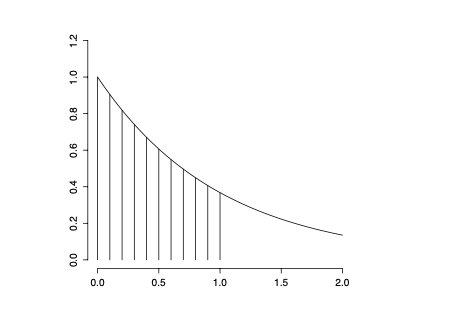
\includegraphics[width=\linewidth]{10_2.png}
    \end{figure}

    \textbf{Punkt 3} - prawdopodobieństwo zdarzenia że $X \in [0,1]$ wynosi
    \begin{align*}
        P(X \in [0,1]) = \int_0^1 f(x) dx = \int_0^1 e^{-x} dx = [-e^{-x}]_{x=0}^{x=1} = 1 - e^{-1}
    \end{align*}


    \subsection{Rozkład normalny}
    \begin{exercise}
        Zmienna losowa X ma rozkład normalny o parametrach $\mu = 0$ oraz $\sigma = 1$. Podaj prawdopodobieństwo, że
        X osiąga wartości dodatnie.
    \end{exercise}
    Rozwiązanie:\\

    Wykres tej funkcji jest parzysty, a pole calego wykresu wynosi 1 więc z połowy jest $\frac{1}{2}$.
    \begin{align*}
        P(X > 0) =  \int_o^{\infty} f(x)dx = \frac{1}{2}
    \end{align*}

    \subsection{Rozkład Gamma, Wzór Gamma-Poisona}
    \begin{exercise}
        Kompilacja programu składa się z 3 części przetwarzanych przez kompilator sekwencyjnie,jedna po drugiej.
        Czas przetwarzania każdej z części ma rozkład wykładniczy ze średnim czasem 5 minut, niezależnym od
        czasu przetwarzania pozostałych części.
        \begin{enumerate}
            \item oblicz wartość oczekiwaną i wariancję całkowitego czasu kompilacji
            \item oblicz prawdopodobieństwo, że cały proces kompilacji zostanie przeprowadzony w
            czasie mniejszym niż 12 minut.
        \end{enumerate}
    \end{exercise}
    Rozwiązanie:\\

    Całkowity czas kompilacji opisuje zmienna losowa o rozkładzie $Gamma(T \sim \Gamma(\alpha = 3, \lambda = \frac{1}{5}))$.
    Wartość oczekiwana i wariancja całkowitego czasu kompilacji to
    \begin{align*}
        E(X) = \frac{\alpha}{\lambda} = \frac{3}{\frac{1}{5}} = 15
    \end{align*}
    \begin{align*}
        Var(x) = \frac{\alpha}{\lambda^2} = \frac{3}{\frac{1}{25}}= 75
    \end{align*}

    Prawdopodobieństwo, że cały proces kompilacji zostanie przeprowadzony w
    czasie mniejszym niż 12 minut liczymy korzystając z formuły Gamma-Poisona.
    \begin{align*}
        P(T < t) = P(X \geq \alpha),
    \end{align*}
    gdzie $X \sim Poisson(\lambda*t = \frac{1}{5} * 12 = 2.4)$ oraz $\alpha = 3$, $t = 12$. Mamy więc:
    \begin{align*}
        P(T < 12) = P (X \geq 3) = 1 - P(0) - P(1) - P(2) = 1 - F_X(2) = 1 - 0.5697 = 0.43
    \end{align*}

    \newpage

    \section{Łancuchy Markowa. Rozkład stacjonarny.}
    \begin{exercise}
        W pewnym mieście każdy dzień jest słoneczny albo deszczowy. Po dniu słonecznym dzień słoneczny
        następuje z prawdopodobieństwem 0.7, a po dniu deszczowym z prawdopodobieństwem 0.4.
        \begin{enumerate}
            \item Narysuj łańcuch markowa oraz wyznacz macierz przejścia dla niego.
            \item W poniedziałek padało. Stwórz prognozę na wtorek, środę i czwartek.
            \item Meteorolodzy przewidują 80\% szans na deszcz w poniedziałek. Stwórz prognozę na wtorek, środę i czwartek.
            \item Znajdź rozkład stacjonarny.
        \end{enumerate}
    \end{exercise}

    \begin{enumerate}
        \item Łańcuch Markowa:
        \begin{center}
            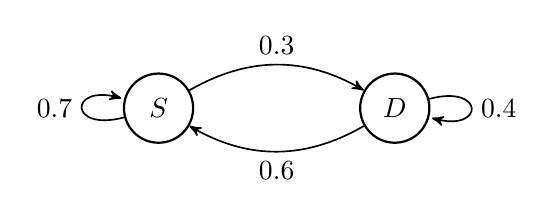
\begin{tikzpicture}[->, >=stealth', auto, semithick, node distance=3cm]
                \tikzstyle{every state}=[fill=white,draw=black,thick,text=black,scale=1]
                \node[state]    (S)                     {$S$};
                \node[state]    (D)[right of=S]   {$D$};
                \path
                (S) edge[loop left]     node{$0.7$}         (S)
                edge[bend left,above]      node{$0.3$}      (D)
                (D) edge[loop right]    node{$0.4$}     (D)
                edge[bend left,below]     node{$0.6$}         (S);
            \end{tikzpicture}

            Macierz przejść:
            \begin{align*}
                \begin{bmatrix}
                    0.7 & 0.3\\
                    0.4 & 0.6
                \end{bmatrix}
            \end{align*}
        \end{center}
        \item \hfill \\
        Wtorek:
        \begin{align*}
            \begin{bmatrix}
                0 & 1
            \end{bmatrix}
            \begin{bmatrix}
                0.7 & 0.3\\
                0.4 & 0.6
            \end{bmatrix}
            =
            \begin{bmatrix}
                0.4 & 0.6
            \end{bmatrix}
        \end{align*}
        Środa:
        \begin{align*}
            \begin{bmatrix}
                0.4 & 0.6
            \end{bmatrix}
            \begin{bmatrix}
                0.7 & 0.3\\
                0.4 & 0.6
            \end{bmatrix}
            =
            \begin{bmatrix}
                0.52 & 0.48
            \end{bmatrix}
        \end{align*}
        Czwartek:
        \begin{align*}
            \begin{bmatrix}
                0.52 & 0.48
            \end{bmatrix}
            \begin{bmatrix}
                0.7 & 0.3\\
                0.4 & 0.6
            \end{bmatrix}
            =
            \begin{bmatrix}
                0.556 & 0.444
            \end{bmatrix}
        \end{align*}
        \item \hfill \\
        Wtorek:
        \begin{align*}
            \begin{bmatrix}
                0.2 & 0.8
            \end{bmatrix}
            \begin{bmatrix}
                0.7 & 0.3\\
                0.4 & 0.6
            \end{bmatrix}
            =
            \begin{bmatrix}
                0.46 & 0.54
            \end{bmatrix}
        \end{align*}
        Środa:
        \begin{align*}
            \begin{bmatrix}
                0.46 & 0.54
            \end{bmatrix}
            \begin{bmatrix}
                0.7 & 0.3\\
                0.4 & 0.6
            \end{bmatrix}
            =
            \begin{bmatrix}
                0.538 & 0.462
            \end{bmatrix}
        \end{align*}
        Czwartek:
        \begin{align*}
            \begin{bmatrix}
                0.538 & 0.462
            \end{bmatrix}
            \begin{bmatrix}
                0.7 & 0.3\\
                0.4 & 0.6
            \end{bmatrix}
            =
            \begin{bmatrix}
                0.5614 & 0.4386
            \end{bmatrix}
        \end{align*}
        \item Macierz przejść:
        \begin{align*}
            \begin{bmatrix}
                0.7 & 0.3\\
                0.4 & 0.6
            \end{bmatrix}
        \end{align*}
        Rozwiązujemy układ równań:
        \begin{align*}
            \left\{\begin{matrix}
                       \pi P = \pi\\
                       \pi_1 + \pi_2 = 1
            \end{matrix}\right.
        \end{align*}
        \begin{align*}
            \pi P =
            \begin{bmatrix}
                \pi_1 & \pi_2
            \end{bmatrix}
            \begin{bmatrix}
                0.7 & 0.3\\
                0.4 & 0.6
            \end{bmatrix}
            =
            \begin{bmatrix}
                0.7\pi_1 + 0.4\pi_2 & 0.3\pi_1 + 0.6\pi_2
            \end{bmatrix}
        \end{align*}
        \begin{align*}
            \left\{\begin{matrix}
                       0.7\pi_1 + 0.4\pi_2 = \pi_1\\
                       0.3\pi_1 + 0.6\pi_2 = \pi_2\\
                       \pi_1 + \pi_2 = 1
            \end{matrix}\right.
        \end{align*}
        Stąd otrzymujemy
        \begin{align*}
            \begin{bmatrix}
                \pi_1 & \pi_2
            \end{bmatrix}
            =
            \begin{bmatrix}
                \frac{4}{7} & \frac{3}{7}
            \end{bmatrix}
        \end{align*}
    \end{enumerate}
    \newpage

    \section{Testy statystyczne: test z, test t-Studenta, test chi-kwadrat.}
    Generalnie:
    \begin{itemize}
        \item Z-testów używamy do sprawdzenia czy testowana próba pasuje do zadanej populacji lub do porównywania dwóch \textbf{dużych} (n $>$ 30) prób
        \item T-testów używamy do porównywania dwóch \textbf{małych} (n $<$ 30) prób testowych ze sobą
        \begin{itemize}
            \item Próby mogą być niezależne - np. wyniki sprawdzianów w dwóch grupach
            \item Mogą być również zależne (dotyczyć jednej i tej samej grupy) - np. waga przed zastosowaniem diety i po
            \item Może również służyć do porównywania próby do zadanej wartości (np. średniej) - podobnie jak Z-testy
        \end{itemize}
        \item Chi-kwadrat używamy do ustalania \texttt{goodness of fit} dla próbki względem populacji lub do zbadania niezależności
    \end{itemize}

    \subsection{Z-test}
    \begin{exercise}
        Inżynier jakości znajduje 10 wadliwych produktów w próbie 500 egzemplarzy pewnego komponentu od wytwórcy A. Wśród 400 egzemplarzy od wytwórcy B znajduje 12 wadliwych. Firma komputerowa, korzystająca z tych komponentów twierdzi, że jakość wyrobów od obu producentów jest taka sama. Sprawdź, czy na 5\% poziomie istotności istnieją wystarczające dowody do odrzucenia tego twierdzenia.
    \end{exercise}

    $H_{0}$: Jakość wyrobów obu producentów jest taka sama \\

    $H_{a}$: Jakość wyrobów obu producentów jest różna \\

    Obliczamy proporcje dla obu prób:
    \begin{equation*}
        p_{1} = \frac{10}{500} = \frac{1}{50}
    \end{equation*}
    \begin{equation*}
        p_{2} = \frac{12}{400} = \frac{3}{100}
    \end{equation*}

    oraz proporcję dla \texttt{próby połączonej}:
    \begin{equation*}
        \bar{p} = \frac{10 + 12}{500 + 400} = \frac{11}{450}
    \end{equation*}

    Następnie używamy wzoru:
    \begin{equation*}
        Z = \frac{p_{1} - p_{2}}{\sqrt{\bar{p}(1-\bar{p})(\frac{1}{n_{1}} + \frac{1}{n_{2}})}}
    \end{equation*}
    \begin{equation*}
        Z = \frac{\frac{1}{50} - \frac{3}{100}}{\sqrt{\frac{11}{450}(1-\frac{11}{450})(\frac{1}{500} + \frac{1}{400})}} = \frac{-\frac{1}{100}}{\sqrt{\frac{4829}{45000000}}} \approx \textbf{\color[HTML]{00ca1f}-0.9653}
    \end{equation*} \\

    W naszej hipotezie mamy pytanie o równość, więc bierzemy pod uwagę obie końcówki przedziału. Mamy sprawdzić prawdziwość naszej hipotezy na 5\% poziomie istotności, więc na każdą końcówkę mamy po 2.5\%. \\

    Odczytujemy z tablic dla Z-testów (tablica rozkładu normalnego) wartość dla \texttt{1 - 0.025 = 0.975} i jest to \textbf{\color[HTML]{b30eff}1.959964} \\

    Następnie odczytujemy z tablic (lub wyliczamy, jeżeli nie mamy tablic z wartościami dla x $<$ 0.5) wartość dla \texttt{0.025} i jest to \textbf{\color[HTML]{b30eff}-1.959964} (po prostu wartość przeciwna do poprzedniej, ponieważ funkcja gęstości rozkładu normalnego jest symetryczna względem środka)

    \begin{figure}[H]
        \center
        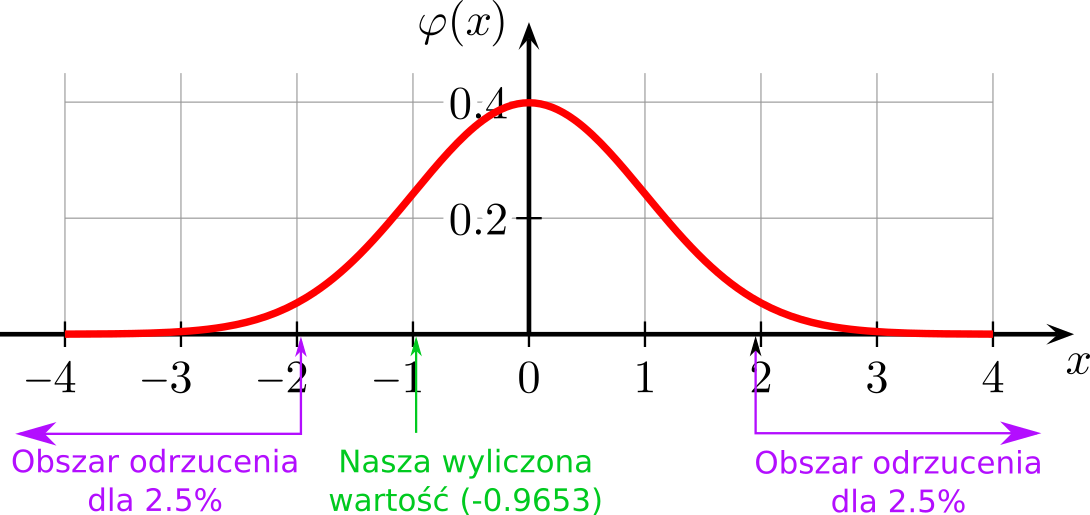
\includegraphics[width=0.7\linewidth]{z-test.png}
    \end{figure}

    Ponieważ nasza wartość nie mieści się w obszarze odrzucenia, nie mamy podstaw do odrzucenia hipotezy zerowej.


    \subsection{T-testy}
    \begin{exercise}
        Posiadacz konta internetowego, w długim okresie czasu, w trakcie logowania pisze swój login i hasło z przerwami pomiędzy kolejnymi wciśnięciami klawiszy wynoszącymi 0.2s. Pewnego dnia zarejestrowane logowanie na to konto z prawidłowym hasłem, przy czym czasy odstępów pomiędzy wciśnięciami kolejnych klawiszy wynosiły: \\

        .24, .22, .26, .34, .35, .32, .33, .29, .19, .36, .30, .15, .17, .20, .28, .40, .37, .27 sekund \\

        Na 5\% poziomie ufności zweryfikuj, czy dane te mogą być dowodem na nieautoryzowany dostęp do konta?
    \end{exercise}

    $H_{0}$: Dostęp do konta jest autoryzowany \\

    $H_{a}$: Dostęp do konta jest nieautoryzowany \\

    Korzystamy ze wzoru:
    \begin{equation*}
        T = \frac{\bar{x} - \mu_{0}}{\sigma}\sqrt{n}
    \end{equation*}

    gdzie:
    \begin{itemize}
        \item $\bar{x}$ - średnia z badanej próby
        \item $\mu_{0}$ - zakładana średnia
        \item $\sigma$ - odchylenie standardowe z próby
        \item n - wielkość próby
    \end{itemize}

    W naszym przypadku:

    \begin{gather}
        \bar{x} \approx 0.28 \\
        \mu_{0} = 0.2 \\
        \sigma \approx 0.07324 \\
        n = 18
    \end{gather}

    Podstawiając do wzoru mamy:
    \begin{equation*}
        T = \frac{0.28 - 0.2}{0.07324}\sqrt{18} \approx \textbf{\color[HTML]{00ca1f}4.63423341}
    \end{equation*}

    Ilość naszych stopni swobody to n-1 więc w naszym przypadku 17 \\

    Odczytujemy z tablic rozkładu t-studenta wartość odpowiadającą 2.5\% poziomowi ufności (5\%/2) oraz 17 stopniom swobody i jest to \textbf{\color[HTML]{b30eff}2.11} oraz wyliczamy tę wartość dla drugiego krańca przedziału (podobnie jak w poprzednim przypadku rozkład t-studenta ma symetryczny wykres względem środka), która jest równa \textbf{\color[HTML]{b30eff}-2.11} \\

    \begin{figure}[H]
        \center
        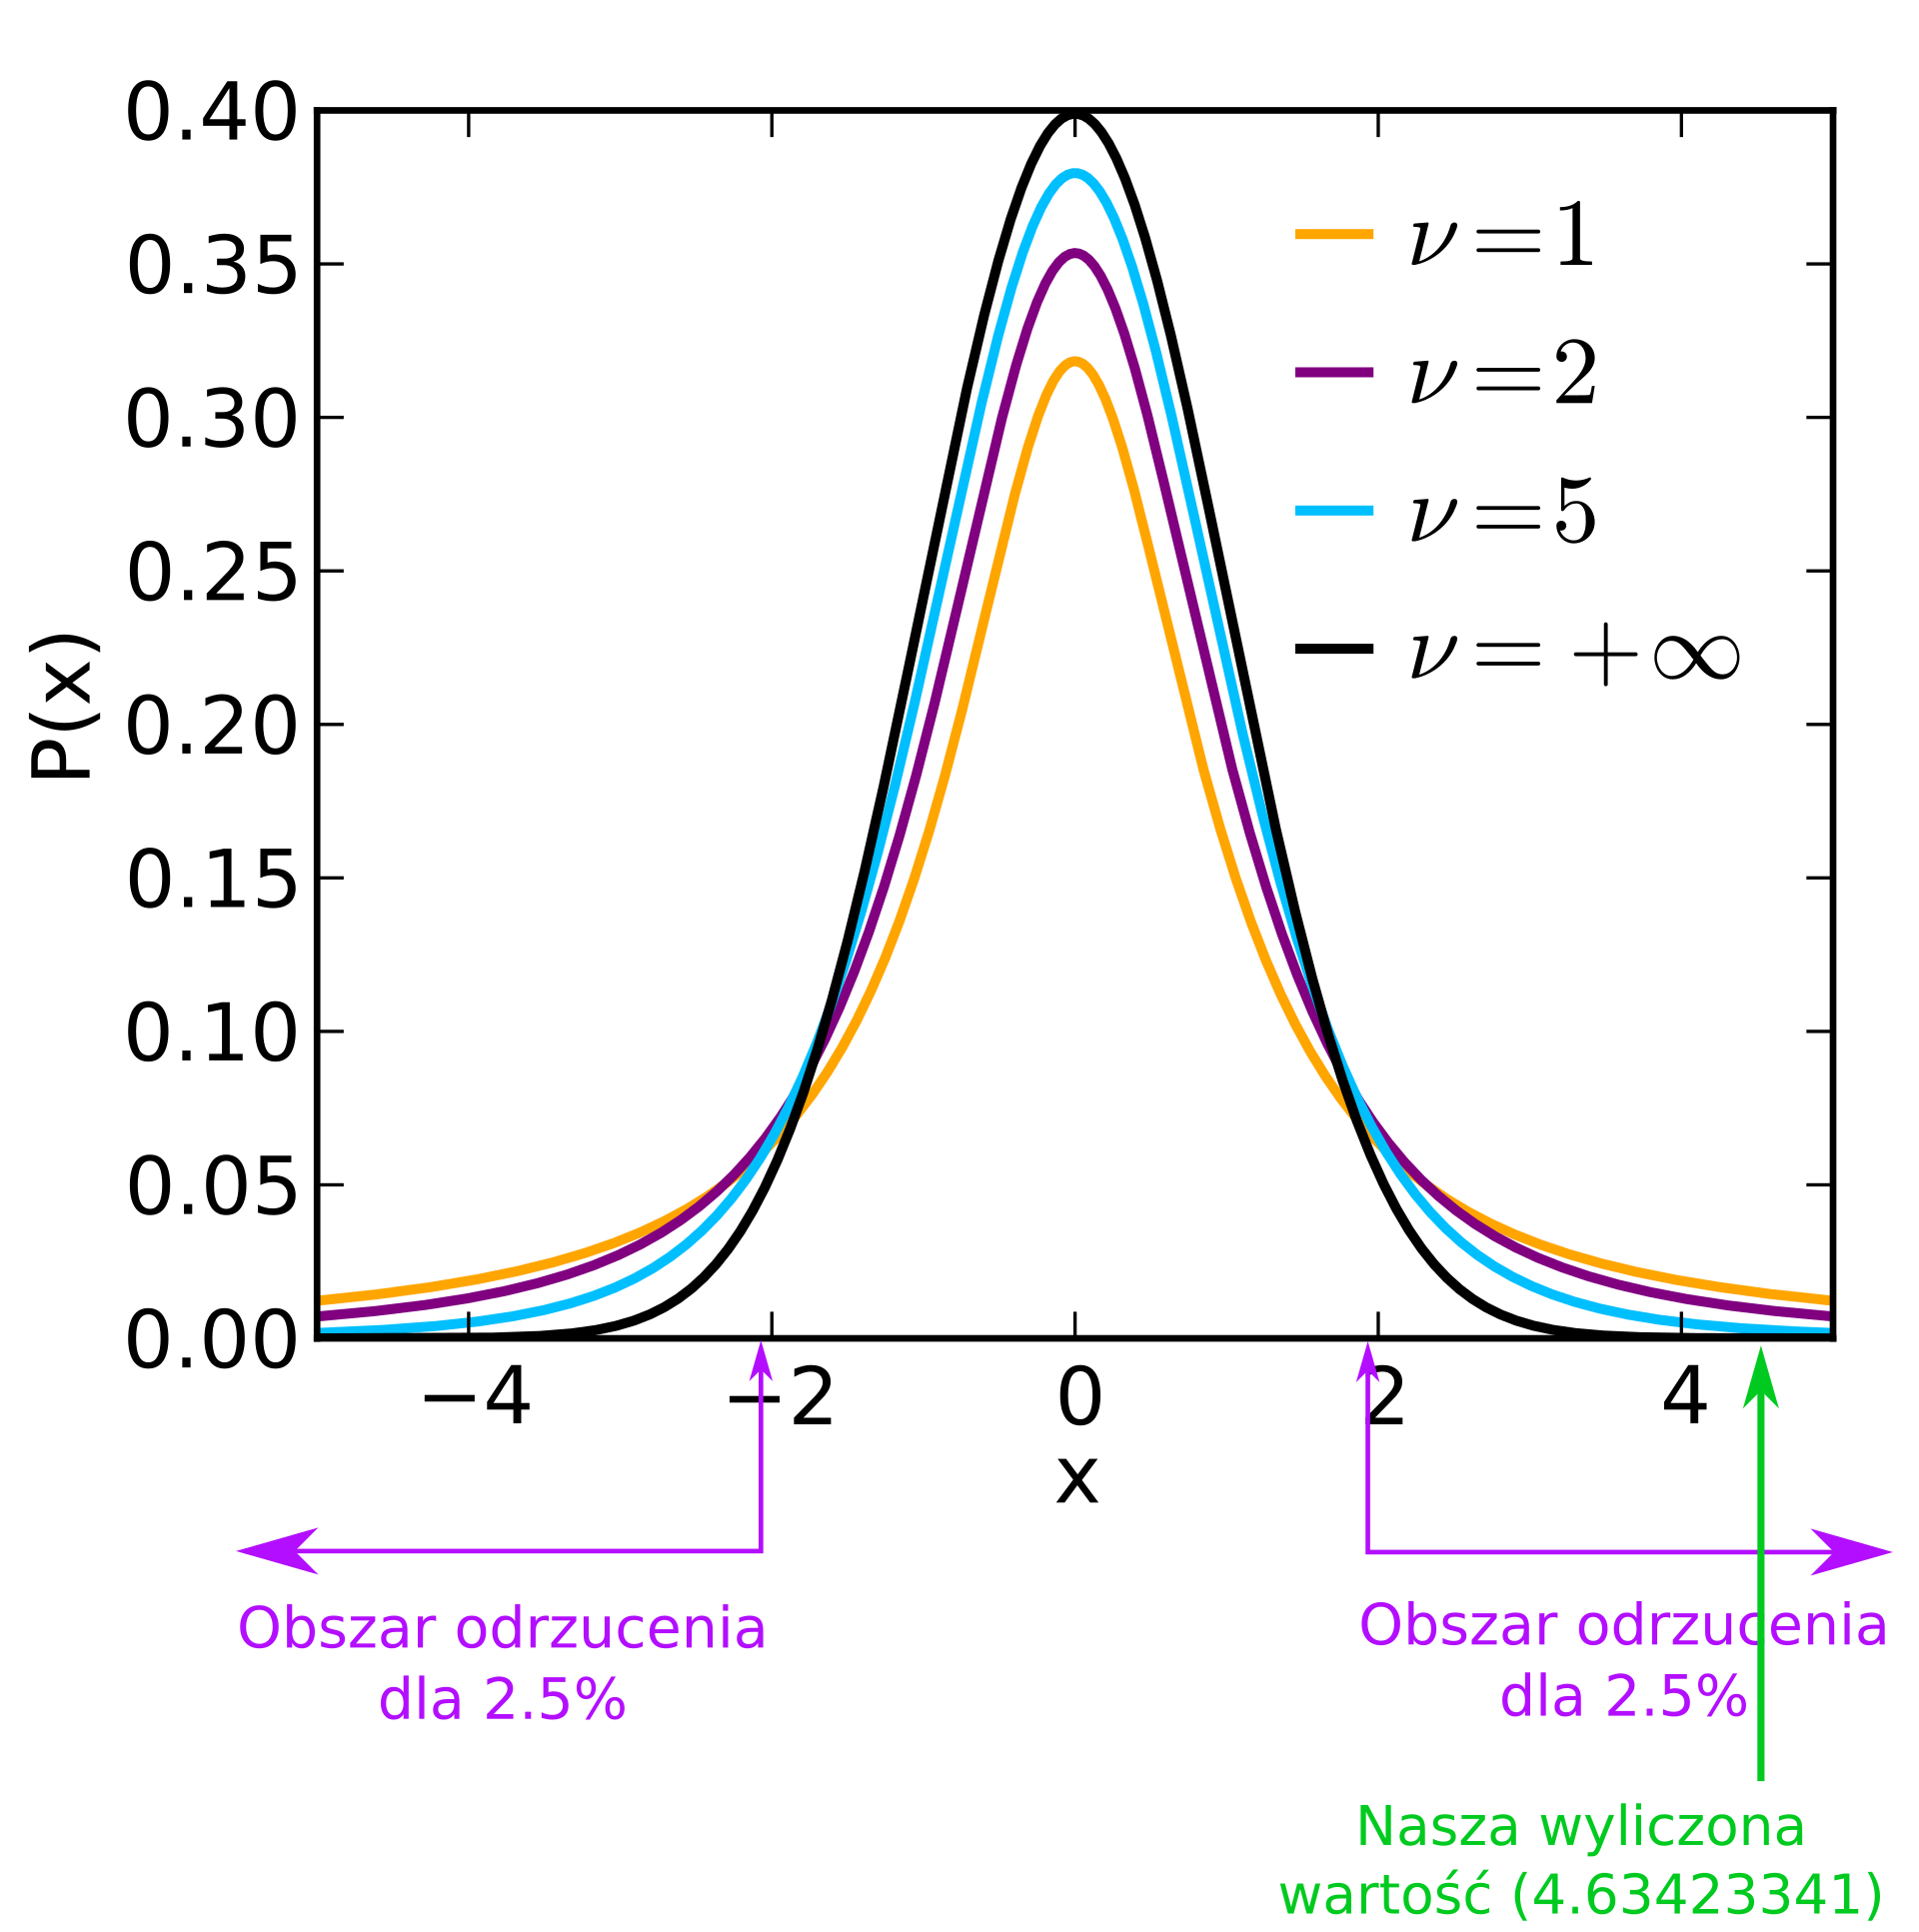
\includegraphics[width=0.7\linewidth]{t-test.png}
    \end{figure}

    Ponieważ 4.63423341 $>$ 2.11 mamy podstawy, aby odrzucić hipotezę zerową i przyjąć hipotezę alternatywną


    \subsection{Testy Chi-kwadrat}
    \begin{exercise}
        Producent kostki do gry deklaruje, że oczka na jego \texttt{niesprawiedliwej} kostce wypadają z następującym prawdopodobieństwem:
        \begin{itemize}
            \item 1 oczko - $\frac{1}{2}$
            \item 2 oczka - $\frac{1}{4}$
            \item 3 oczka - $\frac{1}{25}$
            \item 4 oczka - $\frac{1}{50}$
            \item 5 oczek - $\frac{1}{25}$
            \item 6 oczek - $\frac{3}{20}$
        \end{itemize}
        Dla 100 rzutów zaobserwowano natomiast nastepujące wyniki:
        \begin{itemize}
            \item 1 oczko - 55 razy
            \item 2 oczka - 20 razy
            \item 3 oczka - 6 razy
            \item 4 oczka - 3 razy
            \item 5 oczek - 2 razy
            \item 6 oczek - 14 razy
        \end{itemize}
        Przeprowadź test zgodności (\texttt{goodness of fit}) $\chi^{2}$ i rozstrzygnij na poziomie 5\% istotności, czy producent ma rację
    \end{exercise}

    Wyliczamy wartości oczekiwane dla każdego przedziału i zgodnie z \texttt{rule of thumb} w razie potrzeby je łączymy tak, aby dla każdego z nich wartość była $\geq$ 5

    \begin{table}[H]
        \centering
        \begin{tabular}{|c|c|c|c|c|c|}
            \hline
            n & $Obs_{n}$ & $Exp_{n}$ & x & $Obs_{x}$           & $Exp_{x}$           \\ \hline
            1 & 55 & 50 & 1 & 55 & 50                  \\ \hline
            2 & 20 & 25 & 2 & 20 & 25                  \\ \hline
            3 & 6 & 4 & \multirow{3}{*}{3} & \multirow{3}{*}{11} & \multirow{3}{*}{10} \\ \cline{1-3}
            4 & 3 & 2 & & &                     \\ \cline{1-3}
            5 & 2 & 4 & & &                     \\ \hline
            6 & 14 & 15 & 4 & 14 & 15                  \\ \hline
        \end{tabular}
    \end{table}

    Następnie, aby obliczyć $\chi^{2}$ stosujemy następujący wzór (N to liczba naszych x):
    \begin{equation*}
        \chi^{2} = \sum_{x=1}^{N} \frac{(Obs_{x} - Exp_{x})^{2}}{Exp_{x}}
    \end{equation*}

    W naszym przypadku $\chi^{2} \approx 1.6666$ \\

    Stopnie swobody obliczamy ze wzoru \textbf{N - 1}, gdzie N to liczba naszych x-ów. W naszym przypadku liczba stopni swobody jest więc równa \textbf{3}. \\

    Następnie odczytujemy z tablicy $\chi^{2}$ wartość dla 5\% istotności przy 3 stopniach swobody. Jest ona równa \textbf{7.82} \\

    1.6666 $<$ 7.82 stąd nie mamy więc podstawy do odrzucenia hipotezy zerowej

    \newpage






    \section{Wzór Bayesa i jego interpretacja.}
    \begin{exercise}
        W firmie IT 20\% wytwarzanych modułów przechodzi specjalny proces inspekcji. Z danych historycznych wiadomo, że każdy moduł poddany inspekcji nie ma defektów z prawdopodobieństwem 0.95. Dla modułu nie poddanego procesowi inspekcji prawdopodobieństwo to wynosi jedynie 0.7. Klient znalazł defekt w module. Jakie jest prawdopodobieństwo, że moduł ten przeszedł przez proces inspekcji?
    \end{exercise}

    Korzystamy oczywiście ze wzoru Bayesa:
    \begin{equation*}
        P(A|B) = \frac{P(B|A)P(A)}{P(B)} ~ ~ ~ ~ \text{przy $P(B) > 0$}
    \end{equation*} \\

    I - moduł przeszedł przez inspekcję \\
    D - moduł ma defekt \\

    $P(I) = \frac{20}{100} = \frac{1}{5} ~ ~ ~ ~ P(\bar{I}) = \frac{4}{5}$ \\

    $P(\bar{D}|I) = \frac{95}{100} = \frac{19}{20} ~ ~ ~ ~ P(D|I) = \frac{1}{20}$ \\

    $P(\bar{D}|\bar{I}) = \frac{70}{100} = \frac{7}{10} ~ ~ ~ ~ P(D|\bar{I}) = \frac{3}{10}$ \\

    \begin{equation*}
        P(I|D) = \frac{P(D|I)\cdot P(I)}{P(D)} = \frac{P(D|I)\cdot P(I)}{P(D|I)\cdot P(I) + P(D|\bar{I})\cdot P(\bar{I})} = \frac{\frac{1}{20}\cdot \frac{1}{5}}{\frac{1}{20}\cdot \frac{1}{5} + \frac{3}{10}\cdot \frac{4}{5}} = \frac{1}{25}
    \end{equation*}

    Prawdopodobieństwo, że moduł, w którym znalazł się defekt przeszedł proces inspekcji wynosi $\frac{1}{25}$.

    \newpage
    
    \section{Istnienie elementów odwrotnych względem mnożenia w strukturze $(Zm, +, *)$ w zależności od liczby naturalnej m. Rozszerzony algorytm Euklidesa.}
    \begin{exercise}
    Oblicz element odwrotny do $\mathrm{7}$ w $Z_{19}$.
    %11
    \end{exercise}
    
    $ NWD(7, 19) = 1 $, zatem element odwrotny istnieje
    $$19 / 7 = 2 \;r\; 5$$
    $$7 / 5 = 1 \;r\; 2$$
    $$5 / 2 = 2\; r\; 1$$
	Zatem:
    $$5 = 19 - 2  * 7$$
    $$2 = 7 - 5 = 7 - (19 - 2 * 7) = -19 + 3 * 7$$
    $$1 = 5 - 2 * 2 = 19 - 2 * 7 - 2 * (-19 + 3 * 7) = \mathbf{3} * 19 \mathbf{- 8} * 7$$
    Współczynnik przy 7: $-8$. $-8\; mod\; 19 = 11$\\
    Liczbą odwrotną do 7 w $Z_{19}$ jest 11
    \begin{exercise}
    Oblicz współczynniki Bézouta dla $\mathrm{240}$ i $\mathrm{46}$.
    \end{exercise}
    
    $$240 / 46 = 5 \;r\; 10$$
    $$46 / 10 = 4 \;r\; 6$$
    $$10 / 6 = 1 \;r\; 4$$
    $$6 / 4 = 1 \;r\; 2$$
    $$4 / 2 = 2 \;r\; 0$$
    
    \begin{table}[H]
    \centering
    \begin{tabular}{|c|c|c|c|c|}
    \hline
    $i$ &  $r_i$& $d_i$ &       $x_i$   &       $y_i$       \\
    \hline
    0   &   240 &   -   &       1       &       0           \\
    \hline
    1   &   46  &   5   &       0       &       1           \\
    \hline
    2   &   10  &   4   & 1 - 5 * 0 = 1 & 0 - 5 * 1 = -5    \\
    \hline
    3   &   6   &   1   & 0 - 4 * 1 = -4& 1 - 4 * -5 = 21   \\
    \hline
    4   &   4   &   1   & 1 - 1 * -4 = 5& -5 - 1 * 21 = -26 \\
    \hline
    5   &   2   &   2   &-4 - 1 * 5 = -9& 21 - 1 * -26 = 47 \\
    \hline
    
    \end{tabular}
    \end{table}
    
    $$-9 * 240 + 47 * 46 = 2 = NWD(240, 46)$$
    Współczynniki Bézouta wynoszą -9 i 47.\\
    
    \begin{exercise}
    Pokaż, że jeśli $a, b \in \mathbb{N}$ i $d = NWD(a, b)$ to $\exists m, n : d = ma + nb$.
    \end{exercise}
    
    Mamy zbiór $S = \{ma + nb \; | \; m, n \in \mathbb{Z}, ma + nb > 0\}$. $S$ nie jest puste, zatem (z zasady dobrego uporządkowania) istnieje jego najmniejszy element $d$.
    
    Pokażmy, że $d$ jest dzielnikiem $a$.
    $$a = dq + r$$
    $$r = a - dq$$
    $$r = a - q(ma + nb)$$
    $$r = (1 - qm)a - qnb$$
    $$r = am' + bn'$$
    Zatem $r = 0$ lub $r \in S$. Skoro $r$ jest resztą z dzielenia $a$ przez $d$, to $r < d$. $d$ jest najmniejszym elementem $S$, zatem $r = 0$, zatem $d | a$. Analogiczne rozumowanie możemy przeprowadzić dla $b$.
    
    Pokażmy, że $d = NWD(a, b)$. Niech $c$ będzie wspólnym dzielnikiem $a$ i $b$. Zatem $a = cq_1$ i $b = cq_2$.
    $$d = ma + nb$$
    $$d = cq_1a + cq_2b$$
    $$d = c(q_1a + q_2b)$$
    Zatem $c | d$, zatem $c \leq d$, zatem $d = NWD(a, b)$
    
\section{Ortogonalność wektorów w przestrzeni $R_n$; związki z liniową niezależnością. Metoda ortonormalizacji Grama-Schmidta.}

    \begin{exercise}
    Udowodnij, że każdy ortogonalny układ wektorów jest liniowo niezależny.
    \end{exercise}
    
    Mamy układ wektorów ortogonalnych  $x_1, x_2 ,\dots, x_n$. Zatem $$\forall i,j: i \neq j \; x_i \cdot x_j = 0$$ oraz $$\forall i \; x_i \cdot x_i > 0$$
    Istnieją skalary $a_1, a_2 ,\dots, a_n$, takie, że: $$a_1 * x_1 + a_2 * x_2 + \ldots + a_n * x_n = 0$$
    Powyższe równanie pomnóżmy skalarnie przez $x_1$. 
    $$a_1 * x_1 \cdot x_1 + a_2 * x_2 \cdot x_1 + \ldots + a_n * x_n \cdot x_1 = 0$$
    $$a_1 * x_1 \cdot x_1 + 0 + \ldots + 0 = 0$$
    $$a_1 * x_1 \cdot x_1 = 0$$
    Skoro $x_1 \cdot x_1 > 0$, to $a_1 = 0$. Powyższe działania powtórzmy dla pozostałych wektorów.
    $$a_1 = a_2 = \ldots = a_n = 0$$
    Zatem układ wektorów jest liniowo niezależny.
    \begin{exercise}
    Dokonaj ortonomilizacji wektorów w $\mathbb{R}_3$:             
    
    $\mathbf{v}_1$ =
    $\begin{bmatrix}
    1 & 1 & 0
    \end{bmatrix}
    \mathbf{v}_2 =
    \begin{bmatrix}
    1 & 1 & 1
    \end{bmatrix}
    \mathbf{v}_3 =
    \begin{bmatrix}
    0 & 1 & 1
    \end{bmatrix}$
    \end{exercise}
    
    $$
    \mathbf{u}_1 =
    \begin{bmatrix}
    1 & 1 & 0
    \end{bmatrix}
    $$
    
    $$
    \mathbf{u}_2 =  \mathbf{v}_2 - \mathrm{proj}_\mathbf{u_1} \mathbf{v}_2 = \begin{bmatrix}
    1 & 1 & 1
    \end{bmatrix}
    -
    \frac{2}{2}
    \begin{bmatrix}
    1 & 1 & 0
    \end{bmatrix}
    =
    \begin{bmatrix}
    0 & 0 & 1
    \end{bmatrix}
    $$
    
    $$
    \mathbf{u}_3 =  \mathbf{v}_3 - \mathrm{proj}_\mathbf{u_1} \mathbf{v}_3 - \mathrm{proj}_\mathbf{u_2} \mathbf{v}_3= 
    \begin{bmatrix}
    0 & 1 & 1
    \end{bmatrix}
    -
    \frac{1}{2}
    \begin{bmatrix}
    1 & 1 & 0
    \end{bmatrix}
    -
    \frac{1}{1}
    \begin{bmatrix}
    0 & 0 & 1
    \end{bmatrix}
    =
    \begin{bmatrix}
    -\frac{1}{2} & \frac{1}{2} & 0
    \end{bmatrix}
    $$
    Otrzymane wektory podzielmy przez ich długość:
    $$
    \mathbf{e}_1 =
    \frac
    {\begin{bmatrix}
    1 & 1 & 0
    \end{bmatrix}}
    {\sqrt{2}}
    =
    \begin{bmatrix}
    \frac{\sqrt{2}}{2} & \frac{\sqrt{2}}{2} & 0
    \end{bmatrix}
    $$
    
    $$
    \mathbf{e}_2 =
    \frac
    {\begin{bmatrix}
    0 & 0 & 1
    \end{bmatrix}}
    {1}
    =
    \begin{bmatrix}
    0 & 0 & 1
    \end{bmatrix}
    $$
    
    $$
    \mathbf{e}_3 =
    \frac
    {\begin{bmatrix}
    -\frac{1}{2} & \frac{1}{2} & 0
    \end{bmatrix}}
    {\frac{\sqrt{2}}{2}}
    =
    \begin{bmatrix}
    -\frac{\sqrt{2}}{2} & \frac{\sqrt{2}}{2} & 0
    \end{bmatrix}
    $$

\newpage

    \section{Liczby Stirlinga I i II rodzaju i ich interpretacja.}
    \subsection{Liczby Stirlinga I rodzaju}
    Uzasadnij, że C(4,2)=11\newline 
    Mamy następujące permutacje dwucyklowe zbioru $\{1, 2, 3, 4\}$ \newline

    \begin{center}
    \begin{tabular}{ c c c }
        (1 2)(3 4), (1 3)(2 4), (1 4)(2 3)\\
        (1)(2 3 4), (1)(2 4 3), (2)(1 3 4)\\
        (2)(1 4 3), (3)(1 2 4), (3)(1 4 2)\\
        (4)(1 2 3), (4)(1 3 2) 
    \end{tabular}
    \end{center}
    
    \subsection{Liczby Stirlinga II rodzaju}
    Uzasadnij, że S(4,2) = 7 \newline
    Zbiór $\{1,2,3,4\}$ możemy podzielić na dwa bloki w następujący sposób
    
    \begin{center}
    \begin{tabular}{ c c c }
        \{1\}, \{2, 3, 4\} ; \{2\}, \{1, 3, 4\} ; \{3\}, \{1, 2, 4\} \\
        \{4\}, \{1, 2, 3\} ; \{1, 2\}, \{3, 4\} ; \{1, 3\}, \{2, 4\} \\
        \{1, 4\}, \{2, 3\}
    \end{tabular}
    \end{center}
    \newpage

    \section{Twierdzenia Eulera i Fermata; funkcja Eulera.}
    \subsection{Funkcja Eulera}
    
    \begin{itemize}
        \item $\varphi(2025) = \varphi(3^4 \cdot 5^2) = \varphi(3^4) \cdot \varphi(5^2) = 3^3 \cdot 2 \cdot 5 \cdot 4 = 1080$
        \item $\varphi(1001) = \varphi(7\cdot11\cdot13) = \varphi(7) \cdot \varphi(11) \cdot \varphi(13) = 6 \cdot 10 \cdot12 = 660$
        \item $\varphi(1980) = \varphi(2^2 \cdot 3^2 \cdot 5 \cdot 11) = \varphi(2^2) \cdot \varphi(3^2) \cdot \varphi (5) \cdot \varphi(11) = 2 \cdot 3 \cdot 2 \cdot 4 \cdot 10 = 480$
    \end{itemize}
    
    \subsection{Twierdzenie Fermata}
    
    \subsection{Twierdzenie Eulera}
    \begin{itemize}
        \item Oblicz $2^{64} \pmod {99}$\newline
        NWD(2,99)=1 zatem możemy stosować Twierdzenie Eulera
        
        $\varphi(99) = \varphi(11\cdot 3^2) = \varphi(11) \cdot \varphi(3^2) = 10 \cdot 3 \cdot 2 = 60$
        
        Zatem z Twierdzenia Eulera\newline
        $2^{60} \equiv 1 \pmod {99}$\newline
        $2^{64} = 2^{60} \cdot 2^4 \equiv 2^4 \pmod {99} = 16$
        
        \item Oblicz $99^{400}\pmod {10^3}$\newline
        NWD(99,1000)=1 zatem możemy stosować Twierdzenie Eulera
        
        $\varphi(10^3) = \varphi(2^3 \cdot 5^3) = \varphi(2^3) \cdot \varphi(5^3) = 2^2 \cdot 5^2 \cdot 4 = 400$
        
        Zatem z Twierdzenia Eulera\newline
        $99^{400} \equiv 1 \pmod {10^3}$
        
    \end{itemize}
    \newpage

    \section{Konfiguracje i t-konfiguracje kombinatoryczne.}

    \newpage

    \section{Cykl Hamiltona, obwód Eulera, liczba chromatyczna - definicje i twierdzenia.}

    \newpage

    \section{Algorytm Forda-Fulkersona wyznaczania maksymalnego przepływu.}

    \begin{center}
        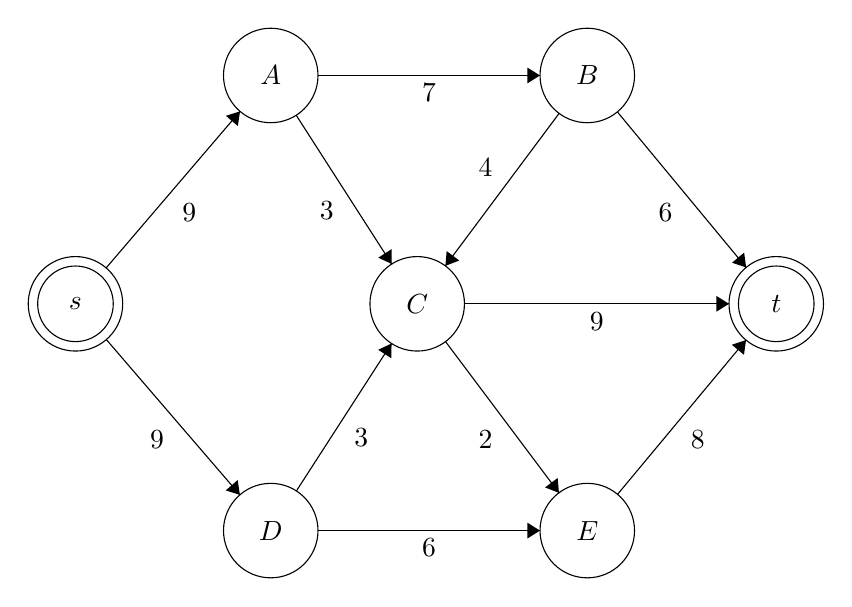
\begin{tikzpicture}[scale=0.2]
            \tikzstyle{every node}+=[inner sep=0pt]
            \draw [black] (12.3,-25.2) circle (3);
            \draw (12.3,-25.2) node {$s$};
            \draw [black] (12.3,-25.2) circle (2.4);
            \draw [black] (24.7,-10.7) circle (3);
            \draw (24.7,-10.7) node {$A$};
            \draw [black] (44.8,-10.7) circle (3);
            \draw (44.8,-10.7) node {$B$};
            \draw [black] (34,-25.2) circle (3);
            \draw (34,-25.2) node {$C$};
            \draw [black] (24.7,-39.6) circle (3);
            \draw (24.7,-39.6) node {$D$};
            \draw [black] (44.8,-39.6) circle (3);
            \draw (44.8,-39.6) node {$E$};
            \draw [black] (56.8,-25.2) circle (3);
            \draw (56.8,-25.2) node {$t$};
            \draw [black] (56.8,-25.2) circle (2.4);
            \draw [black] (14.25,-22.92) -- (22.75,-12.98);
            \fill [black] (22.75,-12.98) -- (21.85,-13.26) -- (22.61,-13.91);
            \draw (19.05,-19.39) node [right] {$9$};
            \draw [black] (27.7,-10.7) -- (41.8,-10.7);
            \fill [black] (41.8,-10.7) -- (41,-10.2) -- (41,-11.2);
            \draw (34.75,-11.2) node [below] {$7$};
            \draw [black] (46.71,-13.01) -- (54.89,-22.89);
            \fill [black] (54.89,-22.89) -- (54.76,-21.95) -- (53.99,-22.59);
            \draw (50.25,-19.38) node [left] {$6$};
            \draw [black] (26.32,-13.23) -- (32.38,-22.67);
            \fill [black] (32.38,-22.67) -- (32.37,-21.73) -- (31.53,-22.27);
            \draw (28.73,-19.26) node [left] {$3$};
            \draw [black] (43.01,-13.11) -- (35.79,-22.79);
            \fill [black] (35.79,-22.79) -- (36.67,-22.45) -- (35.87,-21.85);
            \draw (38.82,-16.56) node [left] {$4$};
            \draw [black] (26.33,-37.08) -- (32.37,-27.72);
            \fill [black] (32.37,-27.72) -- (31.52,-28.12) -- (32.36,-28.66);
            \draw (29.97,-33.71) node [right] {$3$};
            \draw [black] (14.26,-27.47) -- (22.74,-37.33);
            \fill [black] (22.74,-37.33) -- (22.6,-36.39) -- (21.84,-37.05);
            \draw (17.95,-33.85) node [left] {$9$};
            \draw [black] (27.7,-39.6) -- (41.8,-39.6);
            \fill [black] (41.8,-39.6) -- (41,-39.1) -- (41,-40.1);
            \draw (34.75,-40.1) node [below] {$6$};
            \draw [black] (46.72,-37.3) -- (54.88,-27.5);
            \fill [black] (54.88,-27.5) -- (53.98,-27.8) -- (54.75,-28.44);
            \draw (51.35,-33.84) node [right] {$8$};
            \draw [black] (37,-25.2) -- (53.8,-25.2);
            \fill [black] (53.8,-25.2) -- (53,-24.7) -- (53,-25.7);
            \draw (45.4,-25.7) node [below] {$9$};
            \draw [black] (35.8,-27.6) -- (43,-37.2);
            \fill [black] (43,-37.2) -- (42.92,-36.26) -- (42.12,-36.86);
            \draw (38.82,-33.8) node [left] {$2$};
        \end{tikzpicture}
    \end{center}

    Weźmy sobie taką sieć przepływową. Chcemy wyznaczyć jej maksymalny przepływ. Musimy zacząć od jakiegoś (dowolnego)
    przepływu. Szukamy ścieżki rozszerzającej, która połączy źródło s z ujściem t.\\

    Na przykład może to być ścieżka: $P = \{ s  \rightarrow A \rightarrow B \rightarrow t \}$.\\

    Na ścieżce p znajdują się trzy kanały sieci rezydualnej: $(s,A), (A,B) i (B,t)$. Przepustowość rezydualna $c_f(p)$
    ścieżki jest równa najmniejszej przepustowości rezydualnej jej kanałów, czyli przepustowości kanału $(B \rightarrow t)$,
    dla którego $c_f (B,t) = 6$. Zatem wzdłuż krawędzi ścieżki przepływ można zwiększyć o 6 jednostek, o tyle rośnie
    również przepływ sieciowy, czyli $|f_{nowy}| = |f_{stary}| + c_f(p) = 0 + 6 = 6$.\\

    \textbf{Budujemy sieć rezydualną}. Zwiększenie przepływu w kanale sieci pierwotnej o $c_f(p)$ odpowiada
    zmniejszeniu przepustowości rezydualnej tego kanału. Jednocześnie wraz z pojawieniem się przepływu w kanale sieci
    pierwotnej powstaje kanał przeciwny w sieci rezydualnej o przepustowości rezydualnej równej przepływowi.\\

    Przepustowość rezydualna kanału $(s,A)$ wynosi 3 – oznacza to, iż kanałem tym można wciąż jeszcze przesłać trzy
    dodatkowe jednostki przepływu. W sieci rezydualnej pojawia się kanał przeciwny $(A,s)$ o przepustowości rezydualnej
    $c_f(A,s) = 6$.\\

    Kanał $(A,B)$ może jeszcze przesłać 1 dodatkową jednostkę przepływu. Również tutaj pojawił się kanał przeciwny o
    przepustowości rezydualnej równej 6.\\

    Kanał $(B,t)$ przestał istnieć w sieci rezydualnej, ponieważ osiągnął już swoją maksymalną przepustowość – 6
    jednostek przepływu. Nie może on być dalej wykorzystywany do powiększania przepływu. Na jego miejscu mamy
    jednak kanał przeciwny z przepustowością rezydualną równą 6.\\

    \begin{center}
        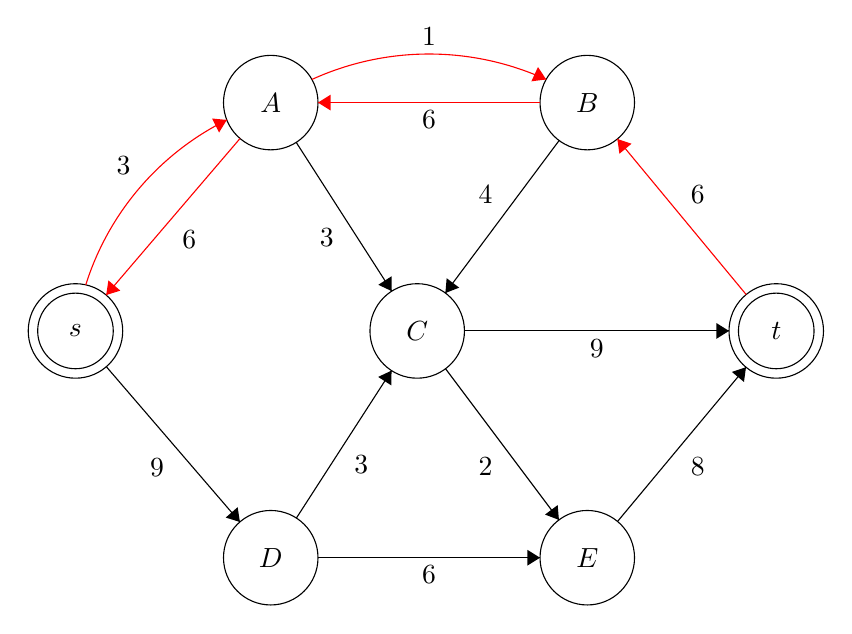
\begin{tikzpicture}[scale=0.2]
            \tikzstyle{every node}+=[inner sep=0pt]
            \draw [black] (12.3,-25.2) circle (3);
            \draw (12.3,-25.2) node {$s$};
            \draw [black] (12.3,-25.2) circle (2.4);
            \draw [black] (24.7,-10.7) circle (3);
            \draw (24.7,-10.7) node {$A$};
            \draw [black] (44.8,-10.7) circle (3);
            \draw (44.8,-10.7) node {$B$};
            \draw [black] (34,-25.2) circle (3);
            \draw (34,-25.2) node {$C$};
            \draw [black] (24.7,-39.6) circle (3);
            \draw (24.7,-39.6) node {$D$};
            \draw [black] (44.8,-39.6) circle (3);
            \draw (44.8,-39.6) node {$E$};
            \draw [black] (56.8,-25.2) circle (3);
            \draw (56.8,-25.2) node {$t$};
            \draw [black] (56.8,-25.2) circle (2.4);
            \draw [red] (12.953,-22.276) arc (162.51949:116.40821:17.599);
            \fill [red] (21.91,-11.8) -- (20.97,-11.71) -- (21.42,-12.6);
            \draw (15.82,-14.68) node [left] {$3$};
            \draw [red] (27.312,-9.232) arc (114.53889:65.46111:17.909);
            \fill [red] (42.19,-9.23) -- (41.67,-8.44) -- (41.25,-9.35);
            \draw (34.75,-7.11) node [above] {$1$};
            \draw [black] (26.32,-13.23) -- (32.38,-22.67);
            \fill [black] (32.38,-22.67) -- (32.37,-21.73) -- (31.53,-22.27);
            \draw (28.73,-19.26) node [left] {$3$};
            \draw [black] (43.01,-13.11) -- (35.79,-22.79);
            \fill [black] (35.79,-22.79) -- (36.67,-22.45) -- (35.87,-21.85);
            \draw (38.82,-16.56) node [left] {$4$};
            \draw [black] (26.33,-37.08) -- (32.37,-27.72);
            \fill [black] (32.37,-27.72) -- (31.52,-28.12) -- (32.36,-28.66);
            \draw (29.97,-33.71) node [right] {$3$};
            \draw [black] (14.26,-27.47) -- (22.74,-37.33);
            \fill [black] (22.74,-37.33) -- (22.6,-36.39) -- (21.84,-37.05);
            \draw (17.95,-33.85) node [left] {$9$};
            \draw [black] (27.7,-39.6) -- (41.8,-39.6);
            \fill [black] (41.8,-39.6) -- (41,-39.1) -- (41,-40.1);
            \draw (34.75,-40.1) node [below] {$6$};
            \draw [black] (46.72,-37.3) -- (54.88,-27.5);
            \fill [black] (54.88,-27.5) -- (53.98,-27.8) -- (54.75,-28.44);
            \draw (51.35,-33.84) node [right] {$8$};
            \draw [black] (37,-25.2) -- (53.8,-25.2);
            \fill [black] (53.8,-25.2) -- (53,-24.7) -- (53,-25.7);
            \draw (45.4,-25.7) node [below] {$9$};
            \draw [black] (35.8,-27.6) -- (43,-37.2);
            \fill [black] (43,-37.2) -- (42.92,-36.26) -- (42.12,-36.86);
            \draw (38.82,-33.8) node [left] {$2$};
            \draw [red] (41.8,-10.7) -- (27.7,-10.7);
            \fill [red] (27.7,-10.7) -- (28.5,-11.2) -- (28.5,-10.2);
            \draw (34.75,-11.2) node [below] {$6$};
            \draw [red] (22.75,-12.98) -- (14.25,-22.92);
            \fill [red] (14.25,-22.92) -- (15.15,-22.64) -- (14.39,-21.99);
            \draw (19.05,-19.39) node [right] {$6$};
            \draw [red] (54.89,-22.89) -- (46.71,-13.01);
            \fill [red] (46.71,-13.01) -- (46.84,-13.95) -- (47.61,-13.31);
            \draw (51.35,-16.52) node [right] {$6$};
        \end{tikzpicture}
    \end{center}

    W nowej sieci rezydualnej szukamy kolejnej ścieżki rozszerzającej:

    \begin{align*}
        P = \{ s \rightarrow A \rightarrow C \rightarrow t \}, ~~~ c_f(p) = 3.
    \end{align*}

    \begin{center}
        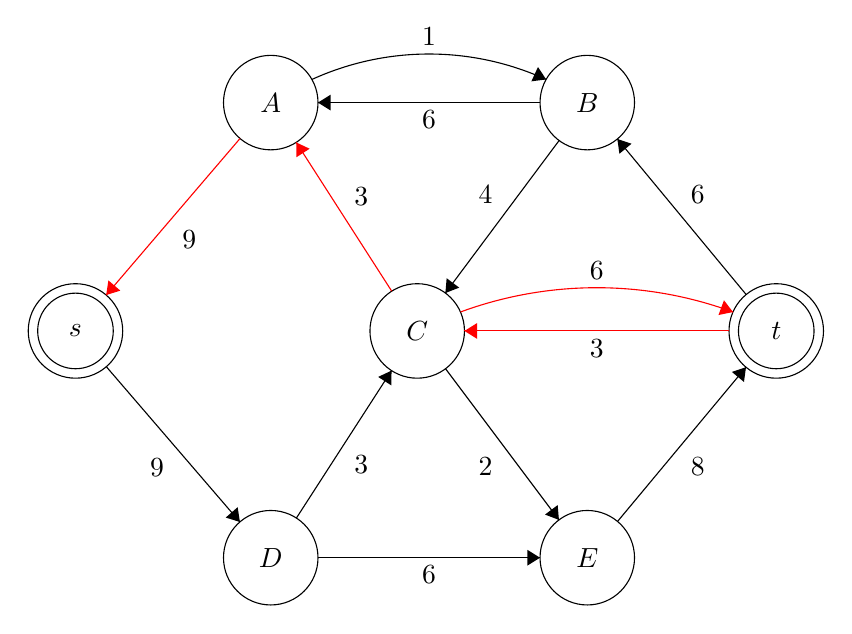
\begin{tikzpicture}[scale=0.2]
            \tikzstyle{every node}+=[inner sep=0pt]
            \draw [black] (12.3,-25.2) circle (3);
            \draw (12.3,-25.2) node {$s$};
            \draw [black] (12.3,-25.2) circle (2.4);
            \draw [black] (24.7,-10.7) circle (3);
            \draw (24.7,-10.7) node {$A$};
            \draw [black] (44.8,-10.7) circle (3);
            \draw (44.8,-10.7) node {$B$};
            \draw [black] (34,-25.2) circle (3);
            \draw (34,-25.2) node {$C$};
            \draw [black] (24.7,-39.6) circle (3);
            \draw (24.7,-39.6) node {$D$};
            \draw [black] (44.8,-39.6) circle (3);
            \draw (44.8,-39.6) node {$E$};
            \draw [black] (56.8,-25.2) circle (3);
            \draw (56.8,-25.2) node {$t$};
            \draw [black] (56.8,-25.2) circle (2.4);
            \draw [black] (27.312,-9.232) arc (114.53889:65.46111:17.909);
            \fill [black] (42.19,-9.23) -- (41.67,-8.44) -- (41.25,-9.35);
            \draw (34.75,-7.11) node [above] {$1$};
            \draw [black] (43.01,-13.11) -- (35.79,-22.79);
            \fill [black] (35.79,-22.79) -- (36.67,-22.45) -- (35.87,-21.85);
            \draw (38.82,-16.56) node [left] {$4$};
            \draw [black] (26.33,-37.08) -- (32.37,-27.72);
            \fill [black] (32.37,-27.72) -- (31.52,-28.12) -- (32.36,-28.66);
            \draw (29.97,-33.71) node [right] {$3$};
            \draw [black] (14.26,-27.47) -- (22.74,-37.33);
            \fill [black] (22.74,-37.33) -- (22.6,-36.39) -- (21.84,-37.05);
            \draw (17.95,-33.85) node [left] {$9$};
            \draw [black] (27.7,-39.6) -- (41.8,-39.6);
            \fill [black] (41.8,-39.6) -- (41,-39.1) -- (41,-40.1);
            \draw (34.75,-40.1) node [below] {$6$};
            \draw [black] (46.72,-37.3) -- (54.88,-27.5);
            \fill [black] (54.88,-27.5) -- (53.98,-27.8) -- (54.75,-28.44);
            \draw (51.35,-33.84) node [right] {$8$};
            \draw [red] (36.746,-23.997) arc (110.22113:69.77887:25.036);
            \fill [red] (54.05,-24) -- (53.48,-23.25) -- (53.13,-24.19);
            \draw (45.4,-21.95) node [above] {$6$};
            \draw [black] (35.8,-27.6) -- (43,-37.2);
            \fill [black] (43,-37.2) -- (42.92,-36.26) -- (42.12,-36.86);
            \draw (38.82,-33.8) node [left] {$2$};
            \draw [black] (41.8,-10.7) -- (27.7,-10.7);
            \fill [black] (27.7,-10.7) -- (28.5,-11.2) -- (28.5,-10.2);
            \draw (34.75,-11.2) node [below] {$6$};
            \draw [red] (22.75,-12.98) -- (14.25,-22.92);
            \fill [red] (14.25,-22.92) -- (15.15,-22.64) -- (14.39,-21.99);
            \draw (19.05,-19.39) node [right] {$9$};
            \draw [black] (54.89,-22.89) -- (46.71,-13.01);
            \fill [black] (46.71,-13.01) -- (46.84,-13.95) -- (47.61,-13.31);
            \draw (51.35,-16.52) node [right] {$6$};
            \draw [red] (32.38,-22.67) -- (26.32,-13.23);
            \fill [red] (26.32,-13.23) -- (26.33,-14.17) -- (27.17,-13.63);
            \draw (29.97,-16.64) node [right] {$3$};
            \draw [red] (53.8,-25.2) -- (37,-25.2);
            \fill [red] (37,-25.2) -- (37.8,-25.7) -- (37.8,-24.7);
            \draw (45.4,-25.7) node [below] {$3$};
        \end{tikzpicture}
    \end{center}

    \noindent Przepływ zwiększamy:
    \begin{align*}
        |f| = 6 + 3 = 9
    \end{align*}
    i modyfikujemy przepustowości rezydualne krawędzi ścieżki rozszerzającej otrzymując nową sieć rezydualną. Znikają z
    niej kanały $(s,A)$ i $(A,C)$ – wykorzystały już swój potencjał zwiększania przepływu.\\

    \noindent Szukamy kolejnej ścieżki rozszerzającej:
    \begin{align*}
        P = \{ s \rightarrow D \rightarrow E \rightarrow t \}, ~~ c_f(p) = 6
    \end{align*}

    \begin{center}
        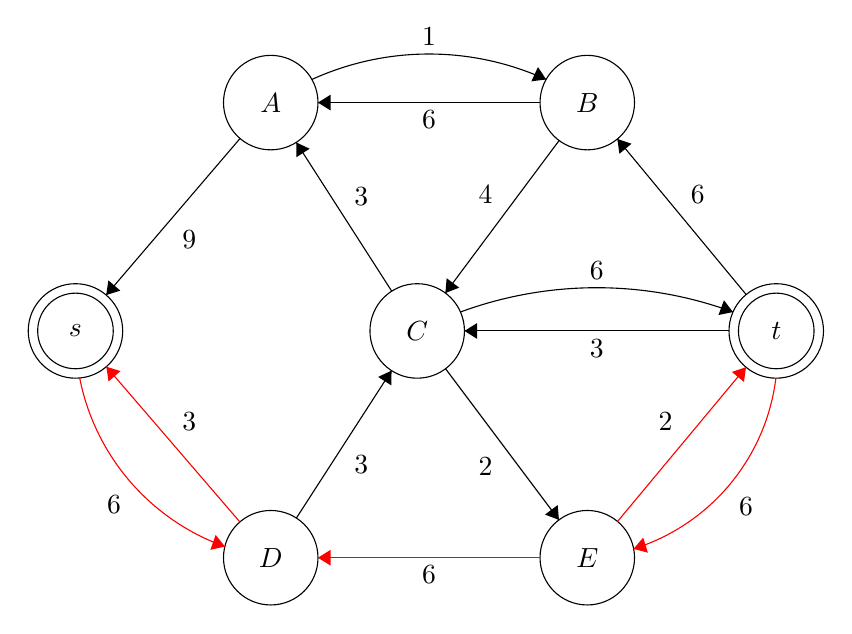
\begin{tikzpicture}[scale=0.2]
            \tikzstyle{every node}+=[inner sep=0pt]
            \draw [black] (12.3,-25.2) circle (3);
            \draw (12.3,-25.2) node {$s$};
            \draw [black] (12.3,-25.2) circle (2.4);
            \draw [black] (24.7,-10.7) circle (3);
            \draw (24.7,-10.7) node {$A$};
            \draw [black] (44.8,-10.7) circle (3);
            \draw (44.8,-10.7) node {$B$};
            \draw [black] (34,-25.2) circle (3);
            \draw (34,-25.2) node {$C$};
            \draw [black] (24.7,-39.6) circle (3);
            \draw (24.7,-39.6) node {$D$};
            \draw [black] (44.8,-39.6) circle (3);
            \draw (44.8,-39.6) node {$E$};
            \draw [black] (56.8,-25.2) circle (3);
            \draw (56.8,-25.2) node {$t$};
            \draw [black] (56.8,-25.2) circle (2.4);
            \draw [black] (27.312,-9.232) arc (114.53889:65.46111:17.909);
            \fill [black] (42.19,-9.23) -- (41.67,-8.44) -- (41.25,-9.35);
            \draw (34.75,-7.11) node [above] {$1$};
            \draw [black] (43.01,-13.11) -- (35.79,-22.79);
            \fill [black] (35.79,-22.79) -- (36.67,-22.45) -- (35.87,-21.85);
            \draw (38.82,-16.56) node [left] {$4$};
            \draw [black] (26.33,-37.08) -- (32.37,-27.72);
            \fill [black] (32.37,-27.72) -- (31.52,-28.12) -- (32.36,-28.66);
            \draw (29.97,-33.71) node [right] {$3$};
            \draw [red] (21.79,-38.893) arc (-109.65577:-168.88001:14.303);
            \fill [red] (21.79,-38.89) -- (21.2,-38.15) -- (20.87,-39.1);
            \draw (15.22,-36.2) node [left] {$6$};
            \draw [red] (46.72,-37.3) -- (54.88,-27.5);
            \fill [red] (54.88,-27.5) -- (53.98,-27.8) -- (54.75,-28.44);
            \draw (50.25,-30.96) node [left] {$2$};
            \draw [black] (36.746,-23.997) arc (110.22113:69.77887:25.036);
            \fill [black] (54.05,-24) -- (53.48,-23.25) -- (53.13,-24.19);
            \draw (45.4,-21.95) node [above] {$6$};
            \draw [black] (35.8,-27.6) -- (43,-37.2);
            \fill [black] (43,-37.2) -- (42.92,-36.26) -- (42.12,-36.86);
            \draw (38.82,-33.8) node [left] {$2$};
            \draw [black] (41.8,-10.7) -- (27.7,-10.7);
            \fill [black] (27.7,-10.7) -- (28.5,-11.2) -- (28.5,-10.2);
            \draw (34.75,-11.2) node [below] {$6$};
            \draw [black] (22.75,-12.98) -- (14.25,-22.92);
            \fill [black] (14.25,-22.92) -- (15.15,-22.64) -- (14.39,-21.99);
            \draw (19.05,-19.39) node [right] {$9$};
            \draw [black] (54.89,-22.89) -- (46.71,-13.01);
            \fill [black] (46.71,-13.01) -- (46.84,-13.95) -- (47.61,-13.31);
            \draw (51.35,-16.52) node [right] {$6$};
            \draw [black] (32.38,-22.67) -- (26.32,-13.23);
            \fill [black] (26.32,-13.23) -- (26.33,-14.17) -- (27.17,-13.63);
            \draw (29.97,-16.64) node [right] {$3$};
            \draw [black] (53.8,-25.2) -- (37,-25.2);
            \fill [black] (37,-25.2) -- (37.8,-25.7) -- (37.8,-24.7);
            \draw (45.4,-25.7) node [below] {$3$};
            \draw [red] (22.74,-37.33) -- (14.26,-27.47);
            \fill [red] (14.26,-27.47) -- (14.4,-28.41) -- (15.16,-27.75);
            \draw (19.05,-30.95) node [right] {$3$};
            \draw [red] (41.8,-39.6) -- (27.7,-39.6);
            \fill [red] (27.7,-39.6) -- (28.5,-40.1) -- (28.5,-39.1);
            \draw (34.75,-40.1) node [below] {$6$};
            \draw [red] (56.777,-28.193) arc (-7.032:-72.57915:13.039);
            \fill [red] (47.74,-39.04) -- (48.65,-39.28) -- (48.35,-38.32);
            \draw (54.41,-36.38) node [right] {$6$};
        \end{tikzpicture}
    \end{center}

    W nowej sieci rezydualnej zniknął kanał $(D,E)$.

    Wciąż jednakże możemy znaleźć nową ścieżkę rozszerzającą:
    \begin{align*}
        P = \{ s  \rightarrow  D \rightarrow C  \rightarrow t \}, ~~~ c_f(p) = 3
    \end{align*}

    \begin{center}
        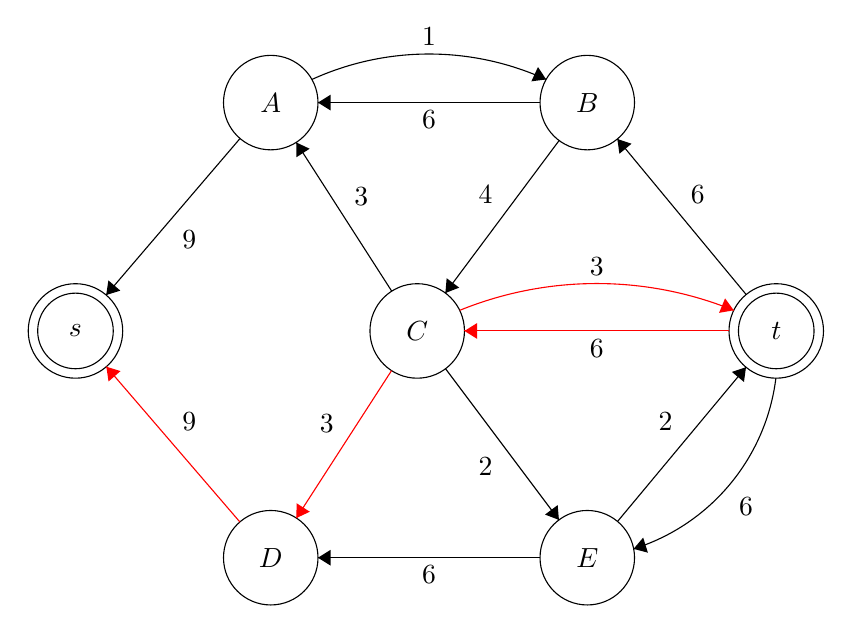
\begin{tikzpicture}[scale=0.2]
            \tikzstyle{every node}+=[inner sep=0pt]
            \draw [black] (12.3,-25.2) circle (3);
            \draw (12.3,-25.2) node {$s$};
            \draw [black] (12.3,-25.2) circle (2.4);
            \draw [black] (24.7,-10.7) circle (3);
            \draw (24.7,-10.7) node {$A$};
            \draw [black] (44.8,-10.7) circle (3);
            \draw (44.8,-10.7) node {$B$};
            \draw [black] (34,-25.2) circle (3);
            \draw (34,-25.2) node {$C$};
            \draw [black] (24.7,-39.6) circle (3);
            \draw (24.7,-39.6) node {$D$};
            \draw [black] (44.8,-39.6) circle (3);
            \draw (44.8,-39.6) node {$E$};
            \draw [black] (56.8,-25.2) circle (3);
            \draw (56.8,-25.2) node {$t$};
            \draw [black] (56.8,-25.2) circle (2.4);
            \draw [black] (27.312,-9.232) arc (114.53889:65.46111:17.909);
            \fill [black] (42.19,-9.23) -- (41.67,-8.44) -- (41.25,-9.35);
            \draw (34.75,-7.11) node [above] {$1$};
            \draw [black] (43.01,-13.11) -- (35.79,-22.79);
            \fill [black] (35.79,-22.79) -- (36.67,-22.45) -- (35.87,-21.85);
            \draw (38.82,-16.56) node [left] {$4$};
            \draw [black] (46.72,-37.3) -- (54.88,-27.5);
            \fill [black] (54.88,-27.5) -- (53.98,-27.8) -- (54.75,-28.44);
            \draw (50.25,-30.96) node [left] {$2$};
            \draw [red] (36.698,-23.892) arc (112.14231:67.85769:23.089);
            \fill [red] (54.1,-23.89) -- (53.55,-23.13) -- (53.17,-24.05);
            \draw (45.4,-21.69) node [above] {$3$};
            \draw [black] (35.8,-27.6) -- (43,-37.2);
            \fill [black] (43,-37.2) -- (42.92,-36.26) -- (42.12,-36.86);
            \draw (38.82,-33.8) node [left] {$2$};
            \draw [black] (41.8,-10.7) -- (27.7,-10.7);
            \fill [black] (27.7,-10.7) -- (28.5,-11.2) -- (28.5,-10.2);
            \draw (34.75,-11.2) node [below] {$6$};
            \draw [black] (22.75,-12.98) -- (14.25,-22.92);
            \fill [black] (14.25,-22.92) -- (15.15,-22.64) -- (14.39,-21.99);
            \draw (19.05,-19.39) node [right] {$9$};
            \draw [black] (54.89,-22.89) -- (46.71,-13.01);
            \fill [black] (46.71,-13.01) -- (46.84,-13.95) -- (47.61,-13.31);
            \draw (51.35,-16.52) node [right] {$6$};
            \draw [black] (32.38,-22.67) -- (26.32,-13.23);
            \fill [black] (26.32,-13.23) -- (26.33,-14.17) -- (27.17,-13.63);
            \draw (29.97,-16.64) node [right] {$3$};
            \draw [red] (53.8,-25.2) -- (37,-25.2);
            \fill [red] (37,-25.2) -- (37.8,-25.7) -- (37.8,-24.7);
            \draw (45.4,-25.7) node [below] {$6$};
            \draw [red] (22.74,-37.33) -- (14.26,-27.47);
            \fill [red] (14.26,-27.47) -- (14.4,-28.41) -- (15.16,-27.75);
            \draw (19.05,-30.95) node [right] {$9$};
            \draw [black] (41.8,-39.6) -- (27.7,-39.6);
            \fill [black] (27.7,-39.6) -- (28.5,-40.1) -- (28.5,-39.1);
            \draw (34.75,-40.1) node [below] {$6$};
            \draw [black] (56.777,-28.193) arc (-7.032:-72.57915:13.039);
            \fill [black] (47.74,-39.04) -- (48.65,-39.28) -- (48.35,-38.32);
            \draw (54.41,-36.38) node [right] {$6$};
            \draw [red] (32.37,-27.72) -- (26.33,-37.08);
            \fill [red] (26.33,-37.08) -- (27.18,-36.68) -- (26.34,-36.14);
            \draw (28.73,-31.09) node [left] {$3$};
        \end{tikzpicture}
    \end{center}

    Przepływ zwiększamy:
    \begin{align*}
        |f| = 15 + 3 = 18.
    \end{align*}

    Po zmodyfikowaniu sieci rezydualnej otrzymujemy nową sieć rezydualną. W tej sieci rezydualnej \textbf{nie znajdziemy już
    żadnej nowej ścieżki rozszerzającej} – ze źródła s nie wychodzi żaden kanał. Oznacza to zakończenie algorytmu, zatem
    znaleźliśmy przepływ maksymalny. Aby otrzymać sieć przepływową wystarczy od przepustowości kanałów odjąć
    otrzymane przepustowości rezydualne – dla nieistniejących kanałów ich przepustowość rezydualna wynosi 0.\\

    \noindent Poniżej nasza sieć przepływowa z uzyskanym maksymalnym przepływem:

    \begin{center}
        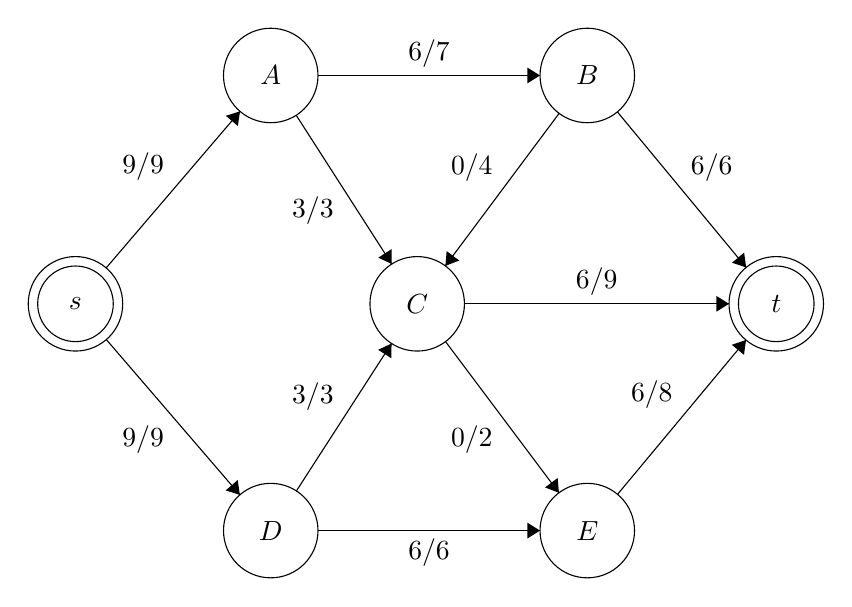
\begin{tikzpicture}[scale=0.2]
            \tikzstyle{every node}+=[inner sep=0pt]
            \draw [black] (12.3,-25.2) circle (3);
            \draw (12.3,-25.2) node {$s$};
            \draw [black] (12.3,-25.2) circle (2.4);
            \draw [black] (24.7,-10.7) circle (3);
            \draw (24.7,-10.7) node {$A$};
            \draw [black] (44.8,-10.7) circle (3);
            \draw (44.8,-10.7) node {$B$};
            \draw [black] (34,-25.2) circle (3);
            \draw (34,-25.2) node {$C$};
            \draw [black] (24.7,-39.6) circle (3);
            \draw (24.7,-39.6) node {$D$};
            \draw [black] (44.8,-39.6) circle (3);
            \draw (44.8,-39.6) node {$E$};
            \draw [black] (56.8,-25.2) circle (3);
            \draw (56.8,-25.2) node {$t$};
            \draw [black] (56.8,-25.2) circle (2.4);
            \draw [black] (27.7,-10.7) -- (41.8,-10.7);
            \fill [black] (41.8,-10.7) -- (41,-10.2) -- (41,-11.2);
            \draw (34.75,-10.2) node [above] {$6/7$};
            \draw [black] (43.01,-13.11) -- (35.79,-22.79);
            \fill [black] (35.79,-22.79) -- (36.67,-22.45) -- (35.87,-21.85);
            \draw (38.82,-16.56) node [left] {$0/4$};
            \draw [black] (46.72,-37.3) -- (54.88,-27.5);
            \fill [black] (54.88,-27.5) -- (53.98,-27.8) -- (54.75,-28.44);
            \draw (50.25,-30.96) node [left] {$6/8$};
            \draw [black] (37,-25.2) -- (53.8,-25.2);
            \fill [black] (53.8,-25.2) -- (53,-24.7) -- (53,-25.7);
            \draw (45.4,-24.7) node [above] {$6/9$};
            \draw [black] (35.8,-27.6) -- (43,-37.2);
            \fill [black] (43,-37.2) -- (42.92,-36.26) -- (42.12,-36.86);
            \draw (38.82,-33.8) node [left] {$0/2$};
            \draw [black] (14.25,-22.92) -- (22.75,-12.98);
            \fill [black] (22.75,-12.98) -- (21.85,-13.26) -- (22.61,-13.91);
            \draw (17.95,-16.51) node [left] {$9/9$};
            \draw [black] (46.71,-13.01) -- (54.89,-22.89);
            \fill [black] (54.89,-22.89) -- (54.76,-21.95) -- (53.99,-22.59);
            \draw (51.35,-16.52) node [right] {$6/6$};
            \draw [black] (26.32,-13.23) -- (32.38,-22.67);
            \fill [black] (32.38,-22.67) -- (32.37,-21.73) -- (31.53,-22.27);
            \draw (28.73,-19.26) node [left] {$3/3$};
            \draw [black] (26.33,-37.08) -- (32.37,-27.72);
            \fill [black] (32.37,-27.72) -- (31.52,-28.12) -- (32.36,-28.66);
            \draw (28.73,-31.09) node [left] {$3/3$};
            \draw [black] (14.26,-27.47) -- (22.74,-37.33);
            \fill [black] (22.74,-37.33) -- (22.6,-36.39) -- (21.84,-37.05);
            \draw (17.95,-33.85) node [left] {$9/9$};
            \draw [black] (27.7,-39.6) -- (41.8,-39.6);
            \fill [black] (41.8,-39.6) -- (41,-39.1) -- (41,-40.1);
            \draw (34.75,-40.1) node [below] {$6/6$};
        \end{tikzpicture}
    \end{center}

    \begin{align*}
        |f| = 18
    \end{align*}



    \newpage

    \section{Rozwiązywanie równan rekurencyjnych przy użyciu funkcji tworzących (generujących) oraz przy użyciu równania charakterystycznego.}

    \subsection{Funkcja tworząca.}

    Przykład
    \begin{align*}
       u_0 = 1, ~ u_1 = 1, ~~ u_{n+2} - 4 u_{n+1} + 4 u_n = 0
    \end{align*}
    \begin{align*}
        u_{n+2} = 4 u_{n+1} - 4 u_n
    \end{align*}
    \begin{align*}
        u_n = 4 u_{n-1} - 4 u_{n-2}
    \end{align*}

    \begin{align*}
        \sum_{n=0}^{\infty} u_n x^n = &1 + 1*x + \sum_{n=2}^{\infty} (4 u_{n-1} - 4 u_{n-2})x^n =\\
        &1 + x + \sum_{n=2}^{\infty} 4 u_{n-1} x^n - \sum_{n=2}^{\infty} 4 u_{n-2} x^n =\\
        &1 + x + 4x \sum_{n=2}^{\infty} u_{n-1} x^{n-1} - 4x^2 \sum_{n=2}^{\infty} u_{n-2} x^{n-2} =\\
        &1 + x + 4x \sum_{n=1}^{\infty} u_n x^n - 4x^2 \sum_{n=0}^{\infty} u_n x^n =\\
        &1 + x + 4x (\sum_{n=0}^{\infty} u_n x^n - u_0) - 4x^2 \sum_{n=0}^{\infty} u_n x^n =\\
        &1 + x - (4x)*1 + 4x \sum_{n=0}^{\infty} u_n x^n - 4x^2 \sum_{n=0}^{\infty} u_n x^n
    \end{align*}

    \begin{align*}
        \sum_{n=0}^{\infty} u_n x^n = 1 - 3x + (4x - 4x^2) \sum_{n=0}^{\infty} u_n x^n
    \end{align*}
    \begin{align*}
        \sum_{n=0}^{\infty} u_n x^n (1 -  4x + 4x^2) = 1 - 3x
    \end{align*}
    \begin{align*}
        \sum_{n=0}^{\infty} u_n x^n (1 -  4x + 4x^2) = 1 - 3x
    \end{align*}
    \begin{align*}
        \sum_{n=0}^{\infty} u_n x^n = \frac{1 - 3x}{1 -  4x + 4x^2} = \frac{1 - 3x}{(1 - 2x)^2}
    \end{align*}
    Rozkład na ułamki proste:
    \begin{align*}
        1 - 3x = A(1 - 2x) + B, ~ 1 = A + B, ~ -3 = -2A, ~~ A = \frac{3}{2}, B = \frac{-1}{2}
    \end{align*}
    Stąd:
    \begin{align*}
        \sum_{n=0}^{\infty} u_n x^n = &\frac{3}{2} * \frac{1}{1 - 2x} - \frac{1}{2} * \frac{1}{(1 - 2x)^2} =\\
        &\frac{3}{2} \sum_{n=0}^{\infty} \binom{n+1-1}{n} (2x)^n - \frac{1}{2} \sum_{n=0}^{\infty} \binom{n+2-1}{n} (2x)^n =\\
        &\frac{3}{2} \sum_{n=0}^{\infty} 2^n x^n - \frac{1}{2} \sum_{n=0}^{\infty} (n+1) 2^n x^n =\\
        &\sum_{n=0}^{\infty} (\frac{3}{2} - \frac{1}{2}(n+1)) 2^n x^n
    \end{align*}
    Więc
    \begin{align*}
        u_n = (\frac{3}{2} - \frac{1}{2}(n+1)) 2^n
    \end{align*}


    \subsection{Równanie charakterystyczne.}
    Przykład 1:
    \begin{align*}
        a_0 = 0, ~ a_1 = 1, ~~ a_{n+2} + a_{n+1} - 2 a_n = 0
    \end{align*}

    Załóżmy, że istnieje rozwiązanie takie, że $a_n = t^n$.
    \begin{align*}
        t^{n+2} + t^{n+1} - 2 t^n = 0
    \end{align*}
    \begin{align*}
        t^2 + t - 2 = 0
    \end{align*}
    \begin{align*}
        \Delta = 1 + 8 = 9
    \end{align*}
    \begin{align*}
        r_1 = \frac{-1 + 3}{2} = 1, ~~ r_2 = \frac{-1 - 3}{2} = -2
    \end{align*}
    Nie jest to pierwiastek podwójny ($r_1 \neq r_2$), zatem wiemy, że:
    \begin{align*}
        \exists C, D: ~~ a_n = C r_1^n + D r_2^n
    \end{align*}
    Podstawiając:
    \begin{align*}
        a_n = C + D (-2)^n
    \end{align*}
    Wyliczamy C i D na podstawie znanych pierwszych wyrazów ciągu:
    \begin{align*}
        a_0 = C + (-2)^0 D = C + D = 0
    \end{align*}
    \begin{align*}
        a_1 = C + (-2)^1 D = C - 2*D = 1
    \end{align*}
    \begin{align*}
        C = \frac{1}{3}, ~~ D = \frac{-1}{3}
    \end{align*}
    \begin{align*}
        a_n = \frac{1}{3} - \frac{(-2)^n}{3} ~ = ~ \frac{1 - (-2)^n}{3}
    \end{align*}

    \hfill \\

    Przykład 2.
    \begin{align*}
        a_0 = -2, ~ a_1 = 1, ~~ a_{n+2} - 2 a_{n+1} + a_n = 0
    \end{align*}
    \begin{align*}
        t^2 - 2t + 1 = 0
    \end{align*}
    \begin{align*}
        (t - 1)^2 = 0
    \end{align*}
    \begin{align*}
        r = r_1 = r_2 = 1
    \end{align*}
    \begin{align*}
        a_n = (C + Dn)r^n
    \end{align*}
    \begin{align*}
        a_0 = (C + D*0)*1^0 = C = -2
    \end{align*}
    \begin{align*}
        a_1 = (C + D*1)*1^1 = C + D = D - 2 = 1
    \end{align*}
    \begin{align*}
        C = -2, ~~ D = 3
    \end{align*}
    \begin{align*}
        a_n = -2 + 3n
    \end{align*}

    \newpage

    \section{Ciąg i granica ciągu liczbowego, granica funkcji.}

    \newpage

    \section{Ciągłość i pochodna funkcji. Definicja i podstawowe twierdzenia.}

    \newpage

    \section{Ekstrema funkcji jednej zmiennej. Definicje i twierdzenia.}

    \newpage

    \section{Całka Riemanna funkcji jednej zmiennej.}

    \newpage

    \section{Pochodne cząstkowe funkcji wielu zmiennych; różniczkowalność i różniczka funkcji.}

    \begin{itemize}
        \item  Korzystając z definicji zbadać, czy istnieją pochodne cząstkowe rzędu pierwszego podanych funkcji
    
        $f(x,y) = x \cdot \sin{xy}, (x_0, y_0) = (\pi,1)$\newline
        \newline
        \begin{equation}
        \begin{aligned}
        \frac{\partial f}{\partial x}(\pi, 1)  \stackrel{def}{=} lim_{\Delta x \rightarrow 0} \frac{f(\pi + \Delta x, 1) - f(\pi, 1)}{\Delta x} = \\
        lim_{\Delta x \rightarrow 0} \frac{(\pi + \Delta x ) \sin{((\pi + \Delta x))} - \pi \sin{(\pi)}}{\Delta x} = \\
        lim_{\Delta x \rightarrow 0} \left[ (\pi + \Delta x) \frac{-sin \Delta x}{\Delta x} \right] = - \pi
        \end{aligned}
        \end{equation}
        
        \item Obliczyć pochodne cząskowe pierwszego rzędu podanych funkcji
        
        $f(x,y) = e^{x^2 \sin y}$\newline
        \newline
        \begin{equation}
            \begin{aligned}
            \frac{\partial f}{\partial x} = \frac{\partial}{\partial x} \left( e^{x^2 \sin y} \right ) = \left( e^{x^2 \sin y} \right) \cdot 2x \sin y
            \end{aligned}
        \end{equation}
        \begin{equation}
            \begin{aligned}
            \frac{\partial f}{\partial y} = \frac{\partial}{\partial y} \left( e^{x^2 \sin y} \right ) = \left( e^{x^2 \sin y} \right) \cdot x^2 \cos y
            \end{aligned}
        \end{equation}
        
        \item Obliczyć pochodne cząstkowe drugiego rzędu podanych funkcji
        
        $f(x,y) = xy + \frac{x^2}{y^3}$
        
        Początkowo wyliczamy pochodne pierwszego rzędu
        \begin{equation}
        \begin{aligned}
        \frac{\partial f}{\partial x} = \frac{\partial }{\partial x} \left( xy + \frac{x^2}{y^3}\right ) = y + \frac{2x}{y^3}
        \end{aligned}
        \end{equation}
        
        \begin{equation}
        \begin{aligned}
         \frac{\partial f}{\partial y} = \frac{\partial }{\partial y} \left( xy + \frac{x^2}{y^3}\right ) = x + \frac{3x^2}{y^4}
         \end{aligned}
        \end{equation}
        
        Następnie wyliczamy pochodne cząstkowe drugiego rzędu
        \begin{equation}
            \begin{aligned}
                \frac{\partial f }{\partial x^2} = \frac{\partial}{\partial x} \left( \frac{\partial f}{\partial x} \right ) = \frac{\partial}{ \partial x} \left( y + \frac{2x}{y^3} \right) = \frac{2}{y^3}
            \end{aligned}
        \end{equation}
        
        \begin{equation}
            \begin{aligned}
                \frac{\partial f }{\partial x \partial y} = \frac{\partial}{\partial x} \left( \frac{\partial f}{\partial y} \right) = \frac{\partial}{\partial x} \left( x - \frac{3x^2}{y^4} \right) = 1 - \frac{6x}{y^4}
            \end{aligned}
        \end{equation}
        
        \begin{equation}
            \begin{aligned}
                \frac{\partial f }{\partial y \partial x} = \frac{\partial}{\partial y} \left( \frac{\partial f}{\partial x} \right) = \frac{\partial}{\partial y} \left( y + \frac{2x}{y^3} \right) = 1 - \frac{6x}{y^4}
            \end{aligned}
        \end{equation}
        
        \begin{equation}
            \begin{aligned}
                \frac{\partial f }{\partial y^2} = \frac{\partial}{\partial y} \left( \frac{\partial f}{\partial y} \right) = \frac{\partial}{\partial y} \left( x - \frac{3x^2}{y^4} \right) = \frac{12x^2}{y^5}
            \end{aligned}
        \end{equation}
        
        \item Korzystajc z definicji zbadać różniczkowalnośc podanych funkcji we wskazanych punktach \newline
        $f(x,y) = x^2 - y^2$
        w punkcie $(x_0, y_0) = (1, -2)$
        
        Korzystając z definicji, wiemy, żę funkcja jest różniczkowalna jeżeli zachodzi poniższa równość
        \begin{equation}
            \lim_{(\Delta x, \Delta y) \rightarrow (0,0)} \frac{f(x_0 + \Delta x, y_0 + \Delta y) - f(x_0, y_0) - \frac{\partial f}{\partial x} (x_0, y_0) \Delta x - \frac{\partial f}{\partial y} (x_0, y_0) \Delta y}{\sqrt{(\Delta x)^2 + (\Delta y)^2}} = 0
        \end{equation}
        
        Najpierw policzymy potrzebne pochodne cząstkowe we wskazanych punktach\newline
        
        $\frac{\partial f}{\partial x} = \frac{\partial }{\partial x} (x^2 - y^2) = 2x \; \; \; \; \; \frac{\partial f}{\partial x} (1,-2) = 2x | _{(1,-2)} = 2 \\$ \newline
        $\frac{\partial f}{\partial y} = \frac{\partial}{\partial y} (x^2 - y^2) = 2y \; \; \; \; \; \frac{\partial f}{\partial y} (1, -2) = 2y | _{(1,-2)} = 4$
        
         Następnie sprawdzimy równość z definicji
         
         \begin{equation}
         \begin{aligned}
            \lim_{(\Delta x, \Delta y) \rightarrow (0,0)} \frac{(1 + \Delta x)^2 - (-2 + \Delta y)^2 - (1 - 4) - 2 \Delta x - 4 \Delta y }{\sqrt{(\Delta x)^2 + (\Delta y)^2}} = \\
            = \lim_{(\Delta x, \Delta y) \rightarrow (0,0)} \frac{1 + 2 \Delta x + (\Delta x)^2 - (4 - 4 \Delta y + (\Delta y)^2) - 2 \Delta x - 4 \Delta y}{ \sqrt{(\Delta x)^2 + (\Delta y)^2}} = \\
            = \lim_{(\Delta x, \Delta y) \rightarrow (0,0)} \frac{(\Delta x)^2 - (\Delta y)^2}{\sqrt{(\Delta x)^2 + (\Delta y)^2}} = \lim_{(\Delta x, \Delta y) \rightarrow (0,0)} \frac{(\Delta x)^2 + (\Delta y)^2 - 2(\Delta y)^2}{\sqrt{(\Delta x)^2 + (\Delta y)^2}} = \\
            = \lim_{(\Delta x, \Delta y) \rightarrow (0,0)} \left[ \sqrt{(\Delta x)^2 + (\Delta y)^2} \right] - \lim_{(\Delta x, \Delta y) \rightarrow (0,0)} \frac{2(\Delta y)^2}{\sqrt{(\Delta x)^2 + (\Delta y)^2}} \\
            \end{aligned}
        \end{equation}
        
        $ \lim_{(\Delta x, \Delta y) \rightarrow (0,0)} \left[ \sqrt{(\Delta x)^2 + (\Delta y)^2} \right] = 0$\newline
        
        Oraz z twierdzenia o trzech ciągach\newline
        \\
        $\lim_{(\Delta x, \Delta y) \rightarrow (0,0)} \frac{2(\Delta y)^2}{\sqrt{(\Delta x)^2 + (\Delta y)^2}} = 0 $\newline
        \\
        Zatem cała granica wynosi 0 oraz funkcja jest różniczkowalna w punkcie (1,-2).
        
        
        
    \end{itemize}
   
    \newpage

    \section{Ekstrema funkcji wielu zmiennych. Definicje i twierdzenia.}
\begin{itemize}
            \item Zbadać czy podana funkcja ma ekstrema lokalne oraz jeśli tak to podać je\\
            
            $f(x,y) = 3(x-1)^2 + 4(y+2)^2 = 3(x^2 - 2x +1) + 4(y^2 + 4y + 4) =\\ = 3x^2 - 6x + 3 + 4y^2 + 16y + 4$\\
            
            Korzystamy z warunku wystarczającego na istnienie ekstremum lokalnego funkcji dwóch zmiennych
            
            Najpierw liczymy pochodne cząstkowe
            
            \begin{equation}
                \begin{aligned}
                    \frac{\partial f}{\partial x} (x,y) = \frac{\partial }{\partial x} \left( 3x^2 - 6x + 3 + 4y^2 + 16y + 4 \right) = 6x - 6 \\
                    \\
                    \frac{\partial f}{\partial y} (x,y) = \frac{\partial }{\partial y} \left( 3x^2 - 6x + 3 + 4y^2 + 16y + 4 \right) = 8y + 16
                \end{aligned}
            \end{equation}
            
            Funkcja f może mieć ekstrema tylko w miejscu zerowania się pochodnych
            
            \begin{equation}
                \begin{aligned}
                    \left \{ \begin{array}{lr}
                                        \frac{\partial f}{\partial x} (x_0, y_0 ) = 0 \\
                                        \\
                                        \frac{\partial f}{\partial y} (x_0, y_0) = 0
                    \end{array} \right.
                    \\
                    \\
                    \left \{ \begin{array}{lr}
                                        6x_0 - 6 = 0 \\
                                        \\
                                        8y_0 + 16 = 0
                    \end{array}\right.
                \end{aligned}
            \end{equation}
            
            Zatem punkt zerowania się pochodnych, w którym funkcja może mieć ekstrema to $P(x_0,y_0) = P(1,-2)$
            
            Wyliczamy pochodne cząstkowe drugiego rzędu oraz badamy znak macierzy Jacobi'ego
            
            \begin{equation}
                \begin{aligned}
                det \begin{bmatrix}
                           \frac{\partial^2 f}{\partial^2 x}(x_0, y_0) & \frac{\partial^2 f}{\partial x \partial y}(x_0, y_0) \\
                           \frac{\partial^2 f}{\partial x \partial y}(x_0, y_0) & \frac{\partial^2 f}{\partial^2 y}(x_0, y_0)
                \end{bmatrix}
                                \end{aligned}
            \end{equation}
            \newpage
         
                 $\frac{\partial f}{\partial x^2} (x,y) = \frac{\partial}{\partial x} \left( 6x - 6 \right) = 6$
                 \\
                 
                $\frac{\partial f}{\partial x \partial y} (x,y)  =  \frac{\partial}{\partial x} \left( 8y + 16 \right) = 0$
                \\
                
                $\frac{\partial f}{\partial y \partial x} (x,y) = \frac{\partial}{\partial y} \left( 6x - 6 \right) = 0$
                \\
                
                $\frac{\partial f}{\partial y^2} (x,y)  = \frac{\partial}{\partial x} \left( 8y + 16 \right) = 8$
                \\
                
                $ det \begin{bmatrix}
                     6 & 0 \\
                     0 & 8
                    \end{bmatrix} = 6 \cdot 8 = 48 > 0$ \\
                    
                Zatem funkcja f ma ekstremum lokalne w punkcie (1,-2) oraz $\frac{\partial f}{\partial x^2}(x_0, y_0) > 0$ zatem jest to minimum lokalne właściwe.

        \end{itemize}
    \newpage

    \section{Twierdzenie o zmianie zmiennych w rachunku całkowym; współrzędne walcowe i sferyczne.}

    \newpage

    \begin{center}
    {\LARGE Teoretyczne podstawy informatyki}
    \end{center}

    \section{Metody dowodzenia poprawności pętli.}
    \section{Odwrotna Notacja Polska: definicja, własności, zalety i wady, algorytmy.}
    \section{Modele obliczen: maszyna Turinga.}
    \section{Modele obliczen: automat skończony, automat ze stosem.}

    \newpage

    \section{Złożoność obliczeniowa - definicja notacji: $O, \Omega, \Theta$.}

    \newpage

    \section{Złożoność obliczeniowa - pesymistyczna i średnia.}

    \newpage

    \section{Metoda "dziel i zwyciężaj"; zalety i wady.}
    \section{Lista: ujęcie abstrakcyjne, możliwe implementacje i ich złożoności.}
    \section{Kolejka i kolejka priorytetowa: ujęcie abstrakcyjne, możliwe implementacje i ich złożoności.}

    \newpage

    \section{Algorytmy sortowania QuickSort i MergeSort: metody wyboru pivota w QS; złożoności.}

    \newpage

    \section{Algorytm sortowania bez porównań (sortowanie przez zliczanie, sortowanie kubełkowe oraz sortowanie pozycyjne).}

    \newpage

    \section{Reprezentacja drzewa binarnego za pomocą porządków (preorder, inorder, postorder).}

    \newpage

    \section{Algorytmy wyszukiwania następnika i poprzednika w drzewach BST; usuwanie węzła.}
    \section{B-drzewa: operacje i ich złożoność.}
    \section{Drzewa AVL: rotacje, operacje z wykorzystaniem rotacji i ich złożoność.}
    \section{Algorytmy przeszukiwania wszerz i w głąb w grafach.}
    \section{Algorytmy wyszukiwania najkrótszej ścieżki (Dijkstry oraz Bellmana-Forda).}
    \section{Programowanie dynamiczne: podział na podproblemy, porównanie z metodą "dziel i zwyciężaj".}
    \section{Algorytm zachłanny: przykład optymalnego i nieoptymalnego wykorzystania.}
    \section{Kolorowania wierzchołkowe (grafów planarnych) i krawędziowe grafów, algorytmy i ich złożoności.}
    \section{Algorytmy wyszukiwania minimalnego drzewa rozpinającego: Boruvki, Prima i Kruskala.}
    \section{Najważniejsze algorytmy wyznaczania otoczki wypukłej zbioru punktów w układzie współrzędnych (Grahama, Jarvisa, algorytm przyrostowy (quickhull)).}
    \section{Problemy P, NP, NP-zupełne i zależności między nimi. Hipoteza P vs. NP.}
    \section{Automat minimalny, wybrany algorytm minimalizacji.}
    \section{Lemat o pompowaniu dla języków regularnych.}
    \section{Warunki równoważne definicji języka regularnego: automat, prawa kongruencja syntaktyczna, wyrażenia regularne.}
    \section{Automaty niedeterministyczne i deterministyczne (w tym ze stosem); determinizacja.}
    \section{Problemy rozstrzygalne i nierozstrzygalne w teorii języków.}
    \section{Klasy języków w hierarchii Chomsky’ego oraz ich zamkniętość ze względu na operacje boolowskie, homomorfizmy, itp.}


    {\Large Wytwarzanie oprogramowania}

    \section{Reprezentacja liczb całkowitych; arytmetyka.}
    \section{Reprezentacja liczb rzeczywistych; arytmetyka zmiennopozycyjna.}
    \section{Różnice w wywołaniu funkcji statycznych, niestatycznych i wirtualnych w C++.}
    \section{Sposoby przekazywania parametrów do funkcji (przez wartość, przez referencję). Zalety i wady.}
    \section{Wskaźniki, arytmetyka wskaźników, różnica między wskaźnikiem a referencją w C++.}
    \section{Podstawowe założenia paradygmatu obiektowego: dziedziczenie, abstrakcja, enkapsulacja, polimorfizm.}
    \section{Funkcje zaprzyjaźnione i ich związek z przeładowaniem operatorów w C++.}
    \section{Programowanie generyczne na podstawie szablonów w języku C++.}
    \section{Podstawowe kontenery w STL z szerszym omówieniem jednego z nich.}
    \section{Obsługa sytuacji wyjątkowych w C++.}
    \section{Obsługa plików w języku C.}
    \section{Model wodospadu a model spiralny wytwarzania oprogramowania.}
    \section{Diagram sekwencji i diagram przypadków użycia w języku UML.}
    \section{Klasyfikacja testów.}
    \section{Model Scrum: struktura zespołu, proces wytwarzania oprogramowania, korzyści modelu.}
    \section{Wymagania w projekcie informatycznym: klasyfikacja, źródła, specyfikacja, analiza.}
    \section{Analiza obiektowa: modele obiektowe i dynamiczne, obiekty encjowe, brzegowe i sterujące.}
    \section{Wzorce architektury systemów.}

    {\Large Inżynieria systemów}

    \section{Relacyjny model danych, normalizacja relacji (w szczególności algorytm doprowadzenia relacji do postaci Boyce’a-Codda), przykłady.}
    \section{Indeksowanie w bazach danych: drzewa B+, tablice o organizacji indeksowej, indeksy haszowe, mapy binarne.}
    \section{Podstawowe cechy transakcji (ACID). Metody sterowania współbieżnością transakcji, poziomy izolacji transakcji, przykłady.}
    \section{Złączenia, grupowanie, podzapytania w języku SQL.}
    \section{Szeregowalność harmonogramów w bazach danych.}
    \section{Definicja cyfrowego układu kombinacyjnego - przykłady układów kombinacyjnych i ich implementacje.}
    \section{Definicja cyfrowego układu sekwencyjnego - przykłady układów sekwencyjnych i ich implementacje.}
    \section{Minimalizacja funkcji logicznych.}
    \section{Programowalne układy logiczne PLD (ROM, PAL, PLA).}
    \section{Schemat blokowy komputera (maszyna von Neumanna).}
    \section{Zarządzanie procesami: stany procesu, algorytmy szeregowania z wywłaszczaniem.}
    \section{Muteks, semafor, monitor jako narzędzia synchronizacji procesów.}
    \section{Pamięć wirtualna i mechanizm stronicowania.}
    \section{Systemy plikowe - organizacja fizyczna i logiczna (na przykładzie wybranego systemu uniksopodobnego).}
    \section{Model ISO OSI. Przykłady protokołów w poszczególnych warstwach.}
    \section{Adresowanie w protokołach IPv4 i IPv6.}
    \section{Najważniejsze procesy zachodzące w sieci komputerowej od momentu wpisania adresu strony WWW do wyświetlenia strony w przeglądarce (komunikat HTTP, segment TCP, system DNS, pakiet IP, ARP, ramka).}
    \section{Działanie przełączników Ethernet, sieci VLAN, protokół STP.}
    \section{Rola routerów i podstawowe protokoły routingu (RIP, OSPF).}
    \section{Szyfrowanie z kluczem publicznym, podpis cyfrowy, certyfikaty.}
    \section{Wirtualne sieci prywatne, protokół IPsec.}


\end{document}
